% !TEX TS-program = xelatex
% !TEX encoding = UTF-8

% This is a simple template for a XeLaTeX document using the "article" class,
% with the fontspec package to easily select fonts.

\documentclass[oneside,10pt]{book} % use larger type; default would be 10pt

% other LaTeX packages.....

%-------------------------------------------------
% Geometry (et sidenotes) : format tufte light
%-------------------------------------------------

\usepackage{sidenotes}

%\usepackage{mwe}

%\usepackage[showframe]{geometry}
\usepackage{geometry}

% option classique
\geometry{letterpaper, left=2cm, right=3in, top=50pt,bottom=50pt, marginparsep=20pt, marginparwidth=2in,  footskip=40pt}

% Option pour faire un document A5
%\geometry{paperwidth=6in, paperheight=9in, left=2cm, right=2in, top=50pt,bottom=50pt, marginparsep=20pt, marginparwidth=1.5in,  footskip=40pt}
 
\renewcommand{\baselinestretch}{1.1} 
\usepackage{placeins} % floatbarrier
\usepackage{fullwidth}
 
\makeatletter
%\renewcommand{\@sidenotes@adjust}{%
% \checkoddpage%
% \ifoddpage%
% %
% \else%
% %\hspace{\@sidenotes@extrawidth}%    %% this was originally there
% \fi}
%%
%% or
%%
\let\@sidenotes@adjust\relax
\makeatother

\setlength\parindent{0pt}
%\usepackage{marginnote}
%\renewcommand*{\raggedleftmarginnote}{}
%\renewcommand*{\raggedrightmarginnote}{}

% Margin Caption (done with sidenotes package)
% UTILISER \sidecaption pour une caption
%\usepackage[margincaption,rightcaption,ragged,wide]{sidecap}
%\usepackage[margincaption,outercaption]{sidecap}
%\sidecaptionvpos{figure}{t} 
%\sidecaptionvpos{table}{t}
% format des captions des figures
%\captionsetup[SCfigure]{format=plain, ...}
%\captionsetup[SCtable]{format=plain, ...}
%-------------------------------------------------
% cadre
%-------------------------------------------------

\usepackage{tikz}
\usepackage[framemethod=TikZ]{mdframed}
\usetikzlibrary{positioning}  
\usepackage{placeins} % FLoatbarrier to force float

\usepackage{xcolor}
%\hypersetup{colorlinks}% uncomment this line if you prefer colored hyperlinks (e.g., for onscreen viewing)
\usepackage{units}
% Typesets the font size, leading, and measure in the form of 10/12x26 pc.


\newcommand{\measure}[3]{#1/#2$\times$\unit[#3]{pc}}
\newcommand{\coefGraph}{1} % Taille du graphe dans les marges; sert uniquement pour Epub, sinon = 1 x textwidth
%\usepackage{multicol} %multicolum for Definition
\newcommand{\largecoefGraph}{1.2} % Taille du graphe dans les marges en proportion de textwidth; sert uniquement pour Epub, sinon = textwidth; remplacer \textwidth par \coefGraph\textwidth
%\usepackage[table]{xcolor}
%\usepackage[xcdraw]{xcolor}
%\usepackage[dvipsnames]{xcolor}
%\usepackage{amsmath,amssymb,amsthm}
%\usepackage{mathtools}
%\usepackage{mathspec}
%\usepackage{xltxtra,xunicode}
\newcommand{\myinnertopmargin}{0pt} % marge qui sert pour les définitions et proprietés




%-------------------------------------------------
% url
%-------------------------------------------------

\usepackage{blindtext}
\usepackage{hyperref}
\usepackage{url}


%-------------------------------------------------
% tableau
%-------------------------------------------------

% pour mettre des tableaux au bon endroit avec l'option H
%\usepackage{float}
% grands tableaux... pratiques
\usepackage{longtable}
 % pour faire des beaux tableaux
\usepackage{booktabs}

 
%-------------------------------------------------
% caractère
%-------------------------------------------------




\usepackage[sc]{mathpazo}
\linespread{1.05}         % Palladio needs more leading (space between lines)

\usepackage{fontspec} % Font selection for XeLaTeX; see fontspec.pdf for documentation
\defaultfontfeatures{Mapping=tex-text} % to support TeX conventions like ``---''


%\setmainfont{Charis SIL} % set the main body font (\textrm), assumes Charis SIL is installed
%\setsansfont{Deja Vu Sans}
%\setmonofont{Deja Vu Mono}

 % format des fonts comme Tufte
 \usepackage{xunicode} % Unicode support for LaTeX character names (accents, European chars, etc)
\usepackage{xltxtra} % Extra customizations for XeLaTeX
\usepackage{amsmath}
\usepackage{amsthm}
% \usepackage{fontspec}
%\setmainfont[Renderer=Basic, Numbers=OldStyle, Scale = 1.0]{TeX Gyre Pagella}
%\setsansfont[Renderer=Basic, Scale=0.90]{TeX Gyre Heros}
%\setmonofont[Renderer=Basic]{TeX Gyre Cursor}
% Palatino for main text and math
%\usepackage[osf,sc]{mathpazo}

% Helvetica for sans serif
% (scaled to match size of Palatino)
%\usepackage[scaled=0.90]{helvet}

% Bera Mono for monospaced
% (scaled to match size of Palatino)
%\usepackage[scaled=0.85]{beramono}
 
%\setmainfont[Numbers=OldStyle, Scale = 1.0]{TeX Gyre Pagella}
%\setsansfont[Scale=0.90]{TeX Gyre Heros}
%\setmonofont{TeX Gyre Cursor}

% pour le chinois
\usepackage{xeCJK}

%-------------------------------------------------
% caractère
%-------------------------------------------------

%\usepackage{biblatex} %pour citer des numero de page
\usepackage[utf8x]{inputenc}

\usepackage[english,main=french]{babel}



\babelprovide[import]{arabic}
\babelfont[arabic]{rm}{Amiri}
\babelprovide[import]{greek}
\babelfont[greek]{rm}{EB Garamond}
% ex
% \foreignlanguage{greek}{Ἰουδαῖοί τε καὶ προσήλυτο.}
%\babelprovide[import]{greek}
%\babelfont[greek]{rm}[RawFeature=+calt]{SimonciniGaramondPro}
\usepackage{arabtex}
%babel-greek
%\usepackage[sc]{mathpazo}

%\linespread{1.05}         % Palladio needs more leading (space between lines)
%\usepackage[T1]{fontenc}
%\renewcommand{\cftsecfont}{\rmfamily\mdseries\upshape}
%\renewcommand{\cftsecpagefont}{\rmfamily\mdseries\upshape} % No bold!

%TARabe dans Name


%Recherche \hypertarget et remplacer par \vide
% \protect\hyperlink par \vide
%\texorpdfstring par RIEN
% \RL : \TArabe
% rechercher \footnote{ et remplacer par \sn{
% rechercher Al Gazali
% package pour faire des réferences à des labels pour le chapitre théologiens
 
%-------------------------------------------------
% bibliography
%-------------------------------------------------

% 
%\usepackage{natbib}
\usepackage{natbib}
\bibliographystyle{unsrtnat}
\bibliographystyle{kluwer}
%\usepackage[notes,backend=biber]{biblatex-chicago}

%\usepackage[style=reading]{biblatex}
%\usepackage[citestyle=reading,bibstyle=authortitle]{biblatex}

%\addbibresource{Theo.bib}

%\bibliography{sample}
%\bibliography{siam}

%\newcommand*{\sidecite}[1]{\sidenote{[\cite{#1}].\citeauthor{#1} - \citetitle{#1}}



 %--------------------------------------------------------------
% Table des matières
%--------------------------------------------------------------
 \usepackage{titletoc}
%%%%% TABLE OF CONTENTS
\setcounter{tocdepth}{1}

\usepackage{etoc}
%%% ToC (table of contents) APPEARANCE
%\usepackage[nottoc,notlof,notlot]{tocbibind} % Put the bibliography in the ToC
%\usepackage[titles,subfigure]{tocloft} % Alter the style of the Table of Contents

\usepackage{cleveref} % referece



\usepackage{eurosym}  %Euro
\usepackage[super]{nth} %for \nth{1} to give 1st
\usepackage{array} % permet de centrer les tableaux\

% Prints the month name (e.g., January) and the year (e.g., 2008)




%\splittopskip=5cm 

 
%-------------------------------------------------
% édition
%-------------------------------------------------
\usepackage{comment}

%-------------------------------------------------
% multi colonnage
%-------------------------------------------------
\usepackage{multicol}





%--------------------------------------------------------------
% Frame
%--------------------------------------------------------------

\usepackage[framemethod=TikZ]{mdframed}

\usepackage{thmtools}
%\usepackage{amsthm}

\usepackage{blindtext} % avoid to cut theorem
% avoid to have theorem or definition in the list of theorm
\makeatletter
\newcommand{\theosep}{\parsep}
\renewcommand{\theosep}{20pt}


%--------------------------------------------------------------
% Titre des listes de théorèmes
%--------------------------------------------------------------

\renewcommand{\listtheoremname}{List of Important Theorems}

\makeatletter
\def\ll@theorem{%
  \protect\numberline{\csname the\thmt@envname\endcsname}%
  \ifx\@empty\thmt@shortoptarg
    \thmt@thmname
  \else
    \thmt@shortoptarg
  \fi}
\def\l@thmt@theorem{} 
 \makeatother
 

% avoid to have theorem or definition in the list of theorm
\makeatletter
\patchcmd\thmt@mklistcmd
  {\thmt@thmname}
  {\check@optarg{\thmt@thmname}}
  {}{}
\patchcmd\thmt@mklistcmd
  {\thmt@thmname\ifx}
  {\check@optarg{\thmt@thmname}\ifx}
  {}{}
\protected\def\check@optarg#1{%
  \@ifnextchar\thmtformatoptarg\@secondoftwo{#1}%
}

 
\makeatother

% format of theorem


            
\declaretheoremstyle[
    headfont=\scshape, 
    notebraces={\scshape : }{.},
    bodyfont=\normalfont,
    headpunct={},
    postheadspace=\newline,
%    postheadhook={\textcolor{red}{\rule[.6ex]{\linewidth}{0.4pt}}\\},
    spacebelow=\parsep,
    spaceabove=\parsep,
    mdframed={
            backgroundcolor=white!20, 
            splittopskip = \topskip,
            linecolor=blue!30, 
            linewidth = 2pt,
            innertopmargin=\myinnertopmargin,
            roundcorner=1pt, 
            innerbottommargin=6pt, 
            skipabove=\parsep,     
            skipbelow=\parsep} 
    ]{Definitionstyle}
    
\declaretheoremstyle[
    headfont=\scshape, 
    notebraces={\scshape : }{.},
    bodyfont=\normalfont,
    headpunct={},
    postheadspace=\newline,
%    postheadhook={\textcolor{red}{\rule[.6ex]{\linewidth}{0.4pt}}\\},
    spacebelow=\parsep,
    spaceabove=\parsep,
    mdframed={backgroundcolor=white!20, 
            splittopskip = \topskip,
            linecolor=red!30, 
            linewidth = 2pt,
            innertopmargin=\myinnertopmargin,
            roundcorner=1pt, 
            innerbottommargin=6pt, 
            skipabove=\parsep,     
            skipbelow=\parsep} 
    ]{Propertystyle}

%,    postfoothook=
% example environment - thmtools
\declaretheoremstyle[
    headfont=\scshape, 
    notebraces={\scshape : }{.},
    bodyfont=\normalfont,
    headpunct={},
    postheadspace=\newline, 
%    postheadhook={\textcolor{red}{\rule[.6ex]{\linewidth}{0.4pt}}\\},
    spacebelow=\parsep,
    spaceabove=\parsep
]{Exercisestyle}
% example environment - thmtools








\declaretheorem[ style = Exercisestyle, numbered=no,name = Property]{property}
\declaretheorem[ style = Propertystyle, name = {Property} ]{Prop}
\declaretheorem[ style = Propertystyle, name = Theorem, sibling=Prop]{Theo}
\declaretheorem[ style = Propertystyle, name = Theorem, sibling=Prop]{theorem}
\declaretheorem[ style = Propertystyle, name = Lemma, sibling=Prop]{lemma}
\declaretheorem[ style = Exercisestyle, numbered=no,name = {Remark}]{rem}
\declaretheorem[ style = Definitionstyle, name = {Definition}]{definition}
\declaretheorem[ style = Definitionstyle, name = {Definition}, sibling=definition]{Def}
\declaretheorem[ style = Exercisestyle, name = Exercise]{exercise}
\declaretheorem[ style = Exercisestyle, name = Exercise, sibling=exercise]{Exercise}
\declaretheorem[ style = Exercisestyle, name = Exercise, sibling=exercise]{Exc}
\declaretheorem[ style = Exercisestyle, name = Exercise, sibling=exercise]{Exo}
\declaretheorem[ style = Exercisestyle, name = Problem, sibling=exercise]{problem}
\declaretheorem[ style = Exercisestyle, name = Example]{example}
\declaretheorem[ style = Exercisestyle, name = Example, sibling=example]{Ex}
\makeatother


%--------------------------------------------------------------
% Code
%--------------------------------------------------------------

%% Permet de mettre du code
\usepackage{listings}
\lstdefinestyle{mystyle}{
    basicstyle=\ttfamily\footnotesize,
    breakatwhitespace=false,         
    breaklines=true,                 
    captionpos=b,                    
    keepspaces=true,                 
    numbers=left,                    
    numbersep=5pt,                  
    showspaces=false,                
    showstringspaces=false,
    showtabs=false,                  
    tabsize=2
}
\lstset{%
	aboveskip=\topsep,
	belowskip=\topsep,
	xleftmargin=\parindent}

\lstset{style=mystyle}





\newcommand{\bi}{\begin{itemize}}
 \newcommand{\ei}{\end{itemize}}
  \newcommand{\be}{\begin{Ex}}
 \newcommand{\ee}{\end{Ex}}
 \newcommand{\mn}[1]{\marginnote{\footnotesize #1}}
  \newcommand{\sn}[1]{\sidenote{\footnotesize #1}}

\newcommand{\mzt}{\emph{muʿtazilite}}  
\newcommand{\CD}{\emph{la Cité de Dieu }}  

\newcommand{\CB}{\emph{Cedric Baylocq }} % nom du professeur
%Recherche \hypertarget et remplacer par \vide
% \protect\hyperlink par \vide
%\texorpdfstring par RIEN
% \RL : \TArabe
% rechercher \footnote{ et remplacer par \sn{
% rechercher Al Gazali
%\newcommand\TArabe[1]{\foreignlanguage{arabic}{\RL}}
\newcommand\TArabe[1]{\foreignlanguage{arabic}{#1}}
\newcommand{\vide}[1]{}

\renewcommand{\listtheoremname}{Liste des Definitions}

% Prints the month name (e.g., January) and the year (e.g., 2008)
\newcommand{\monthyear}{%
  \ifcase\month\or January\or February\or March\or April\or May\or June\or
  July\or August\or September\or October\or November\or
  December\fi\space\number\year
}

\newcommand{\tnote}{\textsuperscript}


% Inserts a blank page
\newcommand{\blankpage}{\newpage\hbox{}\thispagestyle{empty}\newpage}


% Prints an epigraph and speaker in sans serif, all-caps type.
\newcommand{\openepigraph}[2]{%
  %\sffamily\fontsize{14}{16}\selectfont
  \begin{fullwidth}
  \sffamily\large
  \begin{doublespace}
  \noindent\allcaps{#1}\\% epigraph
  \noindent\allcaps{#2}% author
  \end{doublespace}
  \end{fullwidth}
}
 


 

% Prints argument within hanging parentheses (i.e., parentheses that take
% up no horizontal space).  Useful in tabular environments.
\newcommand{\hangp}[1]{\makebox[0pt][r]{(}#1\makebox[0pt][l]{)}}
\newcommand{\hangstar}{\makebox[0pt][l]{*}}
%%
% Prints an asterisk that takes up no horizontal space.
% Useful in tabular environments.



% Macros for typesetting the documentation
\newcommand{\hlred}[1]{\textcolor{Maroon}{#1}}% prints in red
\newcommand{\hangleft}[1]{\makebox[0pt][r]{#1}}
\newcommand{\hairsp}{\hspace{1pt}}% hair space
\newcommand{\hquad}{\hskip0.5em\relax}% half quad space

\newcommand{\ie}{\textit{i.\hairsp{}e.}\xspace}
\newcommand{\eg}{\textit{e.\hairsp{}g.}\xspace}
\newcommand{\na}{\quad--}% used in tables for N/A cells

% Prints an epigraph and speaker in sans serif, all-caps type.





%%
\usepackage{graphicx} % support the \includegraphics command and options

\title{Islam}
\author{Notes du Cours}
%\date{} % Activate to display a given date or no date (if empty),
         % otherwise the current date is printed 

\begin{document}

%\citestyle{verbose}


\maketitle

%-------------------------------------


\pagenumbering{roman} 
\setcounter{page}{1}
\begin{fullwidth}
\tableofcontents
\end{fullwidth}

\pagenumbering{arabic} 
\setcounter{page}{1}
 
\mainmatter

%
\subsubsection{1.1.2 les thématiques des versets
médinois
}

- le thème d'Abraham comme «~Père des croyants~» où Abraham est dit
d'une part \emph{ḥanīf}, c'est-à-dire monothéiste exclusif, mais aussi
\emph{muslim}, c'est-à-dire soumis, abandonné à Dieu, et ni juif ni
chrétien, date de la période médinoise.

(S. 3, 67-68).

«~Abraham n'était ni juif ni chrétien, mais il était un monothéiste
exclusif, abandonné à Dieu~; il n'était pas au nombre des polythéistes.
Les hommes les plus proches d'Abraham sont vraiment ceux qui l'ont
suivi, ainsi que ce Prophète et ceux qui ont cru~».
\marginpar{ \footnotesize This is a margin note using the geometry package, set at 5cm 
vertical offset to the first line it is typeset.}


\foreignlanguage{arabic}{لَكِنْ
}
test
\TArabe{مَا كَانَ إِبْرَاهِيمُ يَهُودِيًّا وَلَا نَصْرَانِيًّا وَلَكِنْ
كَانَ حَنِيفًا مُسْلِمًا وَمَا كَانَ مِنَ الْمُشْرِكِينَ إِنَّ أَوْلَى
النَّاسِ بِإِبْرَاهِيمَ لَلَّذِينَ اتَّبَعُوهُ وَهَذَا النَّبِيُّ
وَالَّذِينَ آَمَنُوا وَاللَّهُ وَلِيُّ الْمُؤْمِنِينَ}




\begin{otherlanguage}{arabic}
{مَا كَانَ إِبْرَاهِيمُ يَهُودِيًّا وَلَا نَصْرَانِيًّا وَلَكِنْ
كَانَ حَنِيفًا مُسْلِمًا وَمَا كَانَ مِنَ الْمُشْرِكِينَ إِنَّ أَوْلَى
النَّاسِ بِإِبْرَاهِيمَ لَلَّذِينَ اتَّبَعُوهُ وَهَذَا النَّبِيُّ
وَالَّذِينَ آَمَنُوا وَاللَّهُ وَلِيُّ الْمُؤْمِنِينَ}
\end{otherlanguage}

Ce verset a bien sûr donné lieu à de multiples commentaires. Il est
souvent interprété dans le sens où Abraham est dépositaire de la
religion originelle avant son altération par les juifs et les chrétiens. \cite{Ben62}
Souvent ne veut pas pour autant dire toujours. Il y a d'autres
lectures\ldots{} \sn{\cite{Ben62}}

\begin{figure}
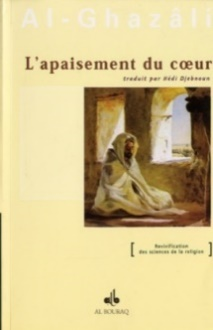
\includegraphics{Images/image002.jpg}
\sidecaption{essai}
\end{figure}


\begin{table}[h!]
\resizebox{\textwidth}{!}{%
\small
\begin{tabular}{p{2cm}p{4cm}p{4cm}}
\toprule
essai & essai & essai \\
\midrule
essai & essai & essai \\
\bottomrule

\end{tabular}%
}
\sidecaption{essai}
\end{table}

\begin{longtable}{p{6cm}p{6cm}}
\toprule
\endhead
«~Quiconque obéit au Messager obéit certainement à Allah~». 
&\TArabe{ مَّن
يُطِعِ الرَّسُولَ فَقَدْ أَطَاعَ اللَّهَ }\\
\bottomrule
\end{longtable}
 \chapter{Introduction}


\mn{Adrien Candiard S2 : 12 heures, 6 semaines, 2 ECTS K. Théologie et connaissance des grandes religions}


L’existence d’une théologie musulmane fait l’objet de mises en doute, parfois chez les penseurs musulmans eux-mêmes, qui soulignent la priorité du droit sur les considérations proprement théologiques. La question théologique, celle du discours humain sur Dieu, a pourtant occupé les savants musulmans de l’époque classique. Le cours visera à faire découvrir ces controverses dont les conséquences sont encore considérables dans tous les domaines des sciences islamiques.


\paragraph{Compétences à acquérir à l’issue de l’enseignement}
\bi
\item Connaître les principales problématiques de la théologie musulmane classique
\item Lire un texte théologique ancien (vocabulaire, notions, style).
\item Thématiser une problématique théologique
\item Acquérir une culture générale théologique
\item Evaluer, à la lumière des connaissances acquises en théologie chrétienne, une démonstration de l’existence de Dieu
\item Faire le lien entre la théologie classique et les problématiques contemporaines
\ei
\paragraph{Sommaire et thèmes}

\bi 
\item Séance 1 : Introduction générale : y a-t-il une théologie musulmane ? 
Les origines du kalām
\item Séance 2 : Le muʿtazilisme
Étude du « credo » muʿtazilite
\item Séance 3 : La réaction ḥanbalite
		Étude d’une profession de foi attribuée à Ibn Ḥanbal
\item Séance 4 : La conciliation ašʿarite
\item Séance 5 : L’ašʿarisme classique 
Étude de la preuve de l’existence de Dieu de Ğuwaynī
\item Séance 6 : La théologie traditionaliste
\ei

\paragraph{Pédagogie et méthodologie (incluant les compléments : TD, numérique, etc.)}




Ouvrages à lire au cours de l’enseignement (5 au maximum)
La bibliographie francophone sur le sujet est malheureusement lacunaire, et datée. On consultera avec profit les deux ouvrages suivants, qui ne sont pas à lire en entier ; des articles ou des chapitres seront indiqués et joints au cours lui-même.
\cite{Gardet:IntroductionTheoMusulmane}


D. GIMARET, Les noms divins en islam, Paris, Cerf, 1988.

\paragraph{Mode d’évaluation}
L’évaluation consistera en un travail de recherche et d’analyse d’environ 10 000 signes.


\chapter{Séance 1 : Introduction générale : y a-t-il une théologie musulmane ? }
\mn{Séquence 1}
Selon Gardet - Anawati\sn{\cite{Gardet:IntroductionTheoMusulmane}, p. 26}
\begin{quote}
    \begin{enumerate}
        \item une période de préformation à Médine
        \item la période de fermentation (ou la rencontre avec la théologie chrétienne - Damas)
        \item la période héroique ; le conflit mu'tazilisme - traditionalisme (ou la rencontre avec la philosophie grecque)
        \item le triomple de l'ash'arisme
        \item l'éclectisme ghazâlien et la voie dite \textit{des modernes}
        \item la période de conservatisme figé
        \item la période de modernisme (ou \textit{réformisme}
    \end{enumerate}
\end{quote}


%------------------------------------------------------------------------------


L'existence même d'une théologie islamique fait aujourd'hui l'objet de
nombreux doutes, aussi bien chez des auteurs d'articles de vulgarisation
sur l'islam que chez beaucoup de musulmans.

Il est pourtant certain qu'il existe, dans les sciences islamiques
classiques, une science appelée en arabe \emph{ʿilm al-kalām} :
\begin{Def}[ʿilm al-kalām]
Littéralement « la science du discours {[}théologique{]} » (plus
vraisemblablement que « science de la Parole {[}divine{]} »). 

On la
désigne également par son contenu essentiel, comme \emph{ʿilm al-tawhīd}
(« science de l'unicité {[}divine{]} »), ou encore, avec des nuances de
sens variant selon les lieux et les temps, \emph{uṣūl al-dīn} (« les
fondements de la religion »). 
\end{Def}

Cette science, avec ses courants, ses
grands noms et ses hérétiques, ses ouvrages de référence, ses
évolutions, ses méthodes propres, a organisé le débat intellectuel au
sein de l'islam essentiellement autour de deux questions essentielles :
\textsc{notre connaissance de Dieu, de sa nature et de ses attributs ; la
liberté de l'homme face à la toute-puissance de Dieu}. Notre cours
s'intéressera au premier chef à la première de ces questions, la plus
directement théologique au sens propre. Puisque cette discipline (le
\emph{ʿilm al-kalām}, ou plus simplement le \emph{kalām}) a existé dans
l'islam médiéval, comment est-il possible que certains affirment que la
théologie islamique n'existe pas ?

Il convient d'abord de remarquer que la science du \emph{kalām}
appartient bien plus à l'histoire de la pensée musulmane qu'à son
actualité, tout au moins dans le monde sunnite. Les penseurs de l'islam
contemporain ne se passionnent guère pour ces débats anciens et
abstraits, et préfèrent en général faire porter leurs efforts sur des
questions plus directement
en prise avec les enjeux d'actualité, comme des débats juridiques
(droits des femmes, droits de l'Homme, statut de la violence...) ou
herméneutiques (comment faut-il lire le Coran et les autres textes de la
tradition islamique ?). On considère couramment, dans le monde arabe,
que le \emph{kalām} est une discipline achevée, qui a trouvé une
solution à toutes les questions qu'elle soulevait et n'est, depuis le
XIVe siècle et la mort d'un de ses derniers représentants, ʿAḍud al-Dīn
al-Īǧī (m. en 1355), qu'un objet de pure curiosité historique. Elle
aurait réglé des problèmes concernant le dogme, mais ne serait pas une
discipline à part entière, d'autant plus inépuisable que son objet est
infini. C'est dans cette optique, celle d'une science achevée, figée,
pour ainsi dire morte, qu'elle est généralement enseignée aujourd'hui.

Il convient aussi de noter que la définition devenue progressivement
classique de l'objet de cette science lui confère une ambition
relativement limitée. C'est le cas de la définition qu'en donne le grand
savant maghrébin du XVe siècle, Ibn Ḫaldūn \label{Theol:IbnKhaldun2}:

\begin{quote}
La science du \emph{kalām} est une science qui fournit les moyens de
prouver les dogmes de la foi par des arguments rationnels, et de réfuter
les innovateurs qui, en ce qui concerne les croyances, s'écartent de la
doctrine suivie par les anciens et par les gens de la tradition.
L'essence même de ces dogmes est la profession de l'unicité de
Dieu.\sn{Ibn Ḫaldūn, \emph{Al-Muqaddima}, voir p. \pageref{theol:IbnKhaldun1}}
\end{quote}

L'objectif ici fixé au \emph{kalām} est essentiellement apologétique et
défensif : il s'agit d'appuyer par des arguments rationnels des dogmes
déjà connus par révélation, et réfuter les hérétiques qui mettent ces
dogmes en doute. Cette science n'est ici qu'instrumentale, au service
d'un catéchisme déjà établi. Elle est très en-deçà des ambitions que le
christianisme médiéval en Occident a attribuées à ses facultés de
théologie, pour qui la théologie conduit à une connaissance effective de
Dieu. Il est d'ailleurs certain que le \emph{kalām} n'a jamais occupé la
place centrale, au sein des sciences islamiques, où trônait la théologie
dans l'Université médiévale d'Occident. Pour autant, il ne faut pas
oublier que la définition donnée par Ibn Ḫaldūn est le fait d'un penseur
qui n'estime guère cette discipline et qui entend ici la dénigrer. Il
n'est pas
lui-même théologien. Les théologiens de l'islam n'auraient probablement
pas donné de leur
science une définition si restrictive.

\begin{Synthesis}
Le kalām s'intéresse à notre connaissance de Dieu, de sa nature et de ses attributs, ainsi qu'à la liberté de l'homme. Question qui n'a jamais été aussi centrale qu'en Occident et qui semble fermée aujourd'hui, défensive, \textit{apologétique} les penseurs de l'islam préférant travailler les questions éthiques.
\end{Synthesis}

\paragraph{Possibilité d'une théologie quand le Coran est la Parole même de Dieu, incréée et sans médiation}
Mais s'élève encore, à l'égard de la théologie islamique, un doute plus
substantiel, plus fondamental. Une théologie au sens propre, une science
qui prendrait Dieu pour objet, est- elle seulement possible en islam ?
La présence d'un texte révélé, le Coran, qui est la Parole même de Dieu,
éternelle et incréée, sans passer par les médiations humaines de
l'inspiration que le christianisme attribue à ses propres Écritures, ne
rend-elle pas vaines toutes les tentatives d'appréhender Dieu par des
raisonnements discursifs ? Une théo-logie, un
« discours rationnel sur Dieu », suppose que la raison peut en dire
quelque chose. Or, ne cesse d'affirmer le Coran, « rien n'est semblable
à Lui » (Coran 42, 11). L'absolue transcendance de Dieu ne le place-t-il
pas très loin de nos approches rationnelles, inaccessible à toutes nos
tentatives ?

Dans sa fameuse conférence donnée à Ratisbonne en septembre 2006, qui ne
portait du reste pas du tout sur l'islam, le pape Benoît XVI s'était, en
introduction, aventuré sur ce terrain\sn{Pour une mise en perspective de cette conférence, voir Ch. Jambet,
2006.}. Citant une controverse
islamo-chrétienne médiévale, il soulignait les conséquences très
concrètes de nos conceptions de Dieu. Si Dieu est accessible à notre
raison, alors nous pouvons en parler, échanger à son sujet des arguments
rationnels, nous employer à nous convaincre réciproquement, sans
recourir à la violence. Si, en revanche, on estime que la nature de Dieu
est par nature inconnaissable, et qu'on ne connaît de lui que sa volonté
(exprimée par révélation), alors la violence est presque inéluctable :
pour étendre une religion, on ne peut faire appel à des arguments
rationnels, et il ne reste que le sabre. À cette analyse fine des
rapports entre la question théologique et la violence, le pape ajoutait,
en citant l'éditeur de la controverse, que pour la doctrine musulmane,
la transcendance de Dieu le rend inaccessible à notre raison. C'est sur
ce dernier point que l'affirmation est discutable. S'il est certain que
l'affirmation de la transcendance de Dieu est un élément central de la
foi
musulmane, \textsc{l'idée que cette transcendance interdit l'entrée de la raison
humaine dans le domaine théologique proprement dit est loin d'avoir fait
consensus chez les auteurs musulmans classiques}. C'est même autour
d'elle que s'organiseront la plupart des débats que nous allons étudier
ici, et l'on constatera que la position selon laquelle la transcendance
divine empêche la raison humaine de s'élever jusqu'à Dieu n'est qu'une
option parmi d'autres chez les musulmans, et une option âprement
discutée au fil des siècles par les théologiens de l'islam, les auteurs
du \emph{kalām}. \textbf{L'effort d'articulation entre la transcendance divine,
si nettement affirmée par la révélation coranique, et les capacités de
la raison humaine constitue le cœur du débat théologique de l'islam
médiéval.}

Ces débats anciens portant sur les capacités du langage humain à dire
Dieu adéquatement, désignés sous le titre classique de « question des
attributs divins » (ou des
«noms divins»), sont souvent abstraits et techniques, mais ils ne sont
nullement inaccessibles pour un lecteur contemporain préparé à les lire
; ils démontrent une inventivité et une liberté d'esprit qui ont de quoi
nous surprendre, si nous les abordons en nous figurant le moyen-âge
comme une époque barbare ou obtuse. Les étudier, comme nous le ferons
ici, c'est découvrir une diversité d'approches bien souvent ignorée
aujourd'hui des musulmans eux-mêmes.

Ce cours sera consacré à la seule période classique, du VIIIe au XIVe
siècle de l'ère chrétienne, c'est-à-dire la période pendant laquelle la
« science du \emph{kalām} » est active. Cela ne signifie pas que la
théologie ait par la suite tout à fait disparu du monde musulman, mais
elle a pris d'autres formes, bien moins systématiques. Le cours sera de
plus essentiellement centré sur le monde sunnite, bien que la frontière
confessionnelle aujourd'hui si nette entre sunnisme et chiisme ait moins
de pertinence pour la période étudiée : des auteurs essentiels, comme le
philosophe Avicenne ou le théologien et scientifique Naṣīr al-Dīn
al-Ṭūsī, étaient chiites, mais leur pensée a exercé une influence qui ne
s'est pas cantonnée au seul monde chiite, loin de là.

L'étude du \emph{kalām} se heurte encore à une autre difficulté pour un
étudiant francophone. Les sources, presque toutes écrites en arabe (ou,
de manière plus exceptionnelle, en persan), ne sont presque jamais
traduites en français, et assez rarement en anglais. Quant aux études
sur le sujet, si l'\emph{Introduction à la théologie musulmane}\sn{\cite{Gardet:IntroductionTheoMusulmane}} de Louis
Gardet et Georges Anawati avait été en 1948 une œuvre pionnière, on ne
dispose plus guère de manuel à jour sur la question en langue française,
et la plupart des études les plus récentes sont publiées en anglais. On
indiquera toutefois pour chaque séquence quelques indications
bibliographiques, privilégiant les ouvrages les plus susceptibles de
vous être accessibles.

L'islam ne naît pas de la spéculation de théologiens subtils. Si le
contexte précis de l'apparition de l'islam nous est très mal connu,
faute de sources historiques fiables\sn{Un point récent sur les débats historiographiques relatifs à l'islam
primitif est proposé dans un petit ouvrage à la fois très bien informé
et très pédagogique, qui permet de s'épargner bien des errances dans un
domaine où l'imagination et l'idéologie fonctionnent à plein : Françoise
Micheau, 2012.}, on sait qu'il naît dans un
contexte à la fois influencé par les débats théologiques de l'Antiquité
tardive et pauvre en culture écrite. Le Coran est certainement marqué
par ces débats, mais ni Muḥammad ni ses compagnons, pas plus que les
conquérants arabes partis au VII\textsuperscript{e} siècle à la conquête
du monde, ne nous ont laissé trace d'une réflexion théologique
discursive. Il faudra plusieurs décennies pour que se formalise une
réflexion de cet ordre et qu'apparaissent les premiers signes de ce que
deviendra la science du \emph{Kalām} ; et de ces débuts, on ne peut
parler qu'avec prudence : si nous connaissons des noms et des courants,
rapportés par des historiens plus tardifs, les textes théologiques
eux-mêmes des époques les plus anciennes ont le plus souvent disparu.
Pour plusieurs de ces courants, on doit se fier aux rapports de leurs
adversaires, ou à des textes mal attribués et probablement écrits bien
plus tard.
\begin{Synthesis}
Le kalām a essayé d'articuler l'affirmation forte de la transcendance divine et de la raison, à travers la question des attributs divins, entre le VIII et XIV.
\end{Synthesis}

\hypertarget{une-origine-interne-ou-externe}{%
\section{Une origine interne ou externe
?}\label{une-origine-interne-ou-externe}}

L'apparition des premières discussions théologiques en islam correspond
à un changement de contexte par rapport à celui de l'apparition de
l'islam. La religion nouvelle est sortie d'Arabie et s'est confrontée,
dans de grands centres urbains très éduqués (Damas, Alexandrie,
Antioche, Ctésiphon...), à des intellectuels chrétiens, juifs ou
mazdéens rompus à la controverse métaphysique et religieuse. Qu'on songe
aux interminables débats qui ont occupé les chrétiens depuis le concile
de Nicée (325), relatifs à la Trinité ou aux deux natures du Christ :
ces querelles ont développé dans l'Église une dialectique très élaborée,
assez
éloignée de la façon très simple qu'a le Coran d'affirmer
l'unicité*\sn{Les mots suivis d'un astérisque font l'objet d'une explicitation dans
le lexique de la séquence (document joint).} de Dieu. Il est donc tentant d'attribuer la
naissance de la théologie islamique à cette rencontre : défiés par des
concurrents redoutablement équipés, les musulmans auraient dû développer
rapidement leur propre système d'argumentation et de défense, qui
donnera naissance à la « science du Kalām ».

Cette hypothèse est séduisante et largement recevable, mais
l'universitaire allemand Josef van Ess, l'une des autorités les plus
considérables dans ce domaine, a relevé ses fragilités\sn{J. van Ess, 1974. Voir aussi J. van Ess, 1977.} : l'examen du
peu de textes anciens dont nous disposons, estime-t-il, ne laisse rien
entrevoir d'une polémique interreligieuse. À cette origine externe et
polémique, il privilégie la piste d'une origine interne : ces débats
naissent naturellement entre les musulmans eux- mêmes, en fonction de
difficultés doctrinales propres à l'islam.

L'historien britannique Michael Cook nuancera bientôt à son tour les
conclusions de Josef van Ess\sn{M. Cook, 1980.}. Il souligne que les textes qu'il évoque
sont très probablement inauthentiques, et qu'il est difficile, en
l'absence de textes assurés, d'opiner dans un sens ou dans l'autre. Cook
remarque en revanche que les manières d'argumenter et d'écrire, très
caractéristiques, qui organiseront la discussion théologique en islam
sont déjà présentes dans des ouvrages de polémiques christologiques
antérieurs à l'islam, en particulier dans le monde chrétien de langue
syriaque. Pour expliquer cette permanence des outils rhétoriques, Cook
propose deux explications qui ne sont d'ailleurs pas exclusives l'une de
l'autre : des musulmans ont pu, en débattant avec les chrétiens, adopter
leur manière d'argumenter ; mais il se peut aussi que des théologiens
chrétiens se soient convertis à l'islam, et aient apporté avec eux leur
manière de débattre et d'écrire.


Sans doute ne faut-il pas chercher à trancher trop nettement entre ces
deux
approches, qui permettent ensemble de rendre compte de la complexité
d'un contexte : la
théologie islamique ne naît pas de rien, et elle est marquée par des
méthodes et des questionnements qui la précèdent ; mais cela ne signifie
nullement qu'elle n'apparaisse que par souci d'imitation. Comme la
théologie chrétienne avait su se saisir d'un outillage philosophique
grec qui la précédait pour faire naître des pensées originales et
profondément chrétiennes, l'islam s'approprie les outils dialectiques et
théologiques qu'il trouve à sa disposition au service d'un
questionnement porté par la révélation coranique.

 
  \subsection{La question du \emph{qadar}}
 

De ce point de vue, il est notable que le premier débat théologique qui
nous soit connu porte sur un embarras que les musulmans trouvent dans la
lecture du Coran. Ce dernier affirme avec force l'absolue
toute-puissance divine, s'opposant ouvertement au fatalisme du paganisme
arabe antéislamique qui plaçait le destin au-dessus des hommes et des
dieux. Mais cette affirmation se heurte bientôt à l'expérience du mal :
en constatant que le mal existe, peut-on tenir à la fois la
toute-puissance et la bonté de Dieu ? N'est-on pas obligé de relativiser
l'un ou l'autre de ces attributs divins ?

Cette question, présente dans tous les monothéismes, prend dans le cas
de l'islam une couleur particulière. Le Coran n'affirme-t-il pas, par
exemple, que
\begin{quote}
    « Dieu guide qui Il veut et égare qui Il veut » (Coran 14,
4) ?
\end{quote} 
Cela signifie-t-il que Dieu est l'auteur du péché de l'homme, que
pourtant il punit des peines de l'Enfer ? À cette question, un
traditionniste de Baṣra, en Irak, Maʿbad ibn ʿAbdallah al-Juhanī (m. en
699) \sn{Ma'bad ibn Abdullah al-Juhani (en arabe : \TArabe{ معبد الجهني}) , mort en 691, appartenait à la tribu des Juhainah qui vivait autour de la ville de Médine. Il a été crucifié par les ordres du calife omeyyade Abd al-Malik à Damas. Il était le premier homme, après Sinbuya, à parler du Qadar (libre arbitre humain).}, va donner une réponse jugée rapidement hétérodoxe : \textsc{Dieu est bien
le créateur de tout ce qui existe, à l'exception toutefois du péché de
l'homme, qui est de sa seule responsabilité.} Pour autant qu'on le sache,
en l'absence de textes de sa plume qui soit parvenu jusqu'à nous, sa
pensée sur le sujet ne semble pas nettement plus élaborée ; elle
n'atteint pas la sophistication que lui donnera bientôt une autre école,
le muʿtazilisme, qui reprendra et développera ces thèses. Il ne semble
pas même qu'il ait construit un système plus général, en s'interrogeant
sur la réciproque : les actes
louables de l'homme lui sont-ils également imputables, ou sont-ils, eux,
à attribuer directement à Dieu ? Il semble que son effort soit plus
théologique (peut-on exonérer Dieu du mal ?) qu'anthropologique (l'homme
est-il responsable de ses actes ?).

Son exécution en 699, probablement due à ses positions hétérodoxes (bien
que l'ensemble des auteurs anciens ne s'accorde pas sur cela),
n'empêchera pas un groupe de penseurs (comme le haut fonctionnaire
Ġaylān al-Dimašqī, qui sera lui aussi exécuté) de tenir et de développer
ces idées, en élaborant une doctrine du libre arbitre de l'homme. Pour
eux, l'homme est responsable de ses actes, qui ne sont donc pas
prédéterminés et décidés par Dieu : l'homme est libre d'agir, de choisir
le bien ou le mal, et c'est ce choix que Dieu jugera au dernier jour.L'homme possède donc un \emph{qadar}.
\begin{Def}[qadar]
Un qadar, c'est-à-dire la faculté ou le
pouvoir de se déterminer soi-même.
\end{Def}
 On appellera donc ses partisans les «
qadarites » --- appellation particulièrement malheureuse, car par la
suite, le mot \emph{qadar} (qui en arabe veut seulement dire « pouvoir») va changer radicalement de signification : il en viendra à désigner
non plus le pouvoir de l'homme de choisir le bien ou le mal, mais au
contraire le pouvoir que Dieu a de déterminer les actions des hommes, la
prédestination, c'est-à-dire précisément ce que les qadarites refusent !

Qu'on ait pu tenir cette position alors qu'elle semble aller contre la
citation coranique citée plus haut (« Dieu guide qui Il veut et égare
qui Il veut ») doit nous inciter à une forme de prudence face à nos
réflexes. Il ne nous appartient évidemment pas de juger de l'orthodoxie
de telle ou telle doctrine : remarquons simplement qu'elles ont existé
au sein de l'islam, à certaines époques, dans certains contextes. De
plus, cela nous amène à remarquer que la lettre du Coran n'est pas si
évidente qu'elle en a l'air quand on le lit en traduction. Des
continuateurs des Qadarites ne manqueront pas de faire remarquer, en
effet, que le verset coranique est susceptible d'une autre lecture,
grammaticalement tout aussi plausible :
\begin{quote}
    « Dieu guide qui le veut {[}=
qui veut être guidé{]} et égare qui le veut {[}= qui veut être égaré{]}
».
\end{quote} 
Cela change évidemment les choses ! On constate ainsi que notre lecture même
du texte coranique
peut dépendre de nos présupposés théologiques\ldots{}

Aucun texte qadarite ne nous est parvenu, si l'on excepte quelques
traités à l'authenticité très controversée\sn{Le plus important d'entre eux est le traité attribué à Ḥasan al-Baṣrī,
\emph{Risālat al-qadar} (« traité sur la prédestination »).}, et il est difficile de
faire la part, dans l'opposition farouche qu'ils ont rencontrée, entre
le refus strictement doctrinal et l'antagonisme politique. Les qadarites
s'impliqueront en effet dans le jeu politique, en particulier au cours
d'une guerre civile qui a divisé l'empire des Omeyyades \sn{(désignée sous
le terme de « troisième \emph{fitna} », qui s'ouvre en 744 et ne
s'achève que par le triomphe d'une nouvelle dynastie, les Abbassides, en
749)} ; l'usurpateur à l'origine de la guerre, le calife Yazīd III, avait
en effet clairement pris parti pour la doctrine qadarite, jusque-là
sévèrement réprimée, et il obtint le soutien de tous ses sympathisants,
mais son échec marquera la fin du mouvement, dont les idées seront
toutefois reprises, de manière plus élaborée, par l'école muʿtazilite.
On a parfois souligné l'impact proprement politique de la doctrine du
libre arbitre, qui aurait menacé l'obéissance aveugle, de droit divin,
exigée par les Omeyyades, mais cette hypothèse est incertaine.

Beaucoup d'auteurs musulmans reprochent aux qadarites d'avoir purement
et simplement adopté la doctrine chrétienne du libre arbitre dans un
contexte musulman, et vont jusqu'à attribuer la doctrine de Maʿbad, le
premier qadarite, à l'enseignement d'un maître chrétien. Cette
affirmation n'est pas aberrante, car confronté à une difficulté
analogue, le christianisme a effectivement développé une nette doctrine
de la liberté d'action de l'être humain ; il ne manquera pas de
reprocher à l'islam sa méconnaissance de cette liberté et sa croyance
fataliste en la prédestination. Pour autant, cette solution n'est pas
nécessairement empruntée au christianisme : elle fait partie des options
possibles devant la difficulté théologique posée par le mal. Et il est
clair que le soupçon d'une origine chrétienne a, sous la plume des
auteurs musulmans qui le rapportent, un objectif polémique : il s'agit
de
montrer que cette doctrine est radicalement étrangère à l'islam
originel, et qu'elle est par conséquent à rejeter comme hétérodoxe.
Cette intention polémique manifeste incite naturellement à la prendre
avec quelques réserves.

Encore mal connu, le mouvement qadarite témoigne néanmoins, dès le
premier siècle de l'islam, de l'émergence d'une réflexion théologique
cherchant à s'organiser, et de réactions énergiques, voire brutales, à
son égard. Mais remarquons que la première naissance de la théologie
islamique s'interroge davantage sur la liberté de l'homme que sur la
nature de Dieu. Cette question n'interviendra que dans un second temps.

\begin{Synthesis}
Le mouvement qadarite est le premier à produire une réflexion théologique, en proposant le \emph{qadar}, la puissance de l'homme de décider en libre arbitre. Néanmoins, le contexte politique (pour le calife Yasid III usurpateur et finalement battu par les abbasides), et une polémique accusant ce mouvement d'être crypto-chrétien l'a fait disparaitre.
\end{Synthesis}
 
 %--------------------------------------------------------------------
\section{Ǧahm Ibn Ṣafwān et la pensée rationnelle en
théologie} 
\label{Theol:JahmIbnSafwan}

Un autre nom doit être cité dans cette préhistoire de la théologie
musulmane : celui de Ǧahm Ibn Ṣafwān\sn{Aussi translittéré Jahm ibn Ṣafwān \TArabe{ (جَهْم بن صَفْوان)} } (m. en 746), actif dans les mêmes
décennies que le mouvement qadarite mais dans une tout autre région de
l'empire, son extrémité orientale, le Ḫurāsān (région correspondant à
l'est de l'Iran et l'Afghanistan). Personnage mal connu, dont aucun
écrit ne nous est parvenu et sur lequel tout notre savoir vient de ses
très nombreux adversaires, Ǧahm est, de l'avis général, le premier
auteur à avoir présenté la pensée rationnelle (\emph{ʿaql}) comme un
moyen de parvenir à des vérités théologiques, pouvant conduire à
corriger des lectures jugées trop littérales du texte coranique.

\begin{Def}[Neoplatonisme]
doctrine philosophique de l’Antiquité tardive, élaborée notamment
par le philosophe égyptien de langue grecque Plotin (IIIe
siècle ap. J.-C.), qui réalise une
synthèse des pensées de Platon et d’Aristote autour d’une réflexion métaphysique et
mystique prônant le retour à l’Un divin. C’est à partir de cette doctrine que s’élaborera
d’abord la falsafa, ou « philosophie islamique ».
\end{Def}
Plusieurs auteurs, anciens et contemporains, soulignent l'influence de
la philosophie grecque sur la pensée de Ǧahm. Cette influence, en
particulier celle du néoplatonisme* de l'Antiquité tardive, est
incontestable, mais elle ne doit pas occulter la pensée profondément
originale développée par le théologien persan, qui s'affranchit très
volontiers des cadres philosophiques reçus (comme la distinction
aristotélicienne essentielle de la substance et de l'accident). On a
aussi noté qu'il reçoit l'héritage des discussions patristiques
chrétiennes, en particulier sur les questions trinitaires. Sur une
question qui prendra, comme nous le verrons, une grande ampleur par la
suite, Ǧahm s'appuie explicitement sur des débats qu'il mène
contre des chrétiens : il affirme que \textsc{le Coran, Parole de Dieu, est créé
et non pas éternel, par souci de cohérence }; en effet, pour la foi
musulmane, le Christ, que le Coran qualifie de
« Parole et Esprit de Dieu » (Coran 4, 171), est une créature, donc le
Coran lui-même doit l'être aussi. Affirmer l'éternité du Coran, ce
serait risquer de donner raison aux chrétiens qui affirment que le
Christ est davantage qu'une créature.

Par les œuvres de ses adversaires, nous connaissons un grand nombre de
thèses de Ǧahm Ibn Ṣafwān, mais hors de leur contexte et sans
continuité. Retrouver la cohérence de son œuvre est un travail minutieux
qui provoque beaucoup de débats entre les chercheurs, et il n'est pas
question d'en examiner ici le détail. On peut en revanche retenir qu'il
identifie le premier le point névralgique qui ne cessera d'occuper la
théologie musulmane dans les siècles qui suivront. Le Coran,
remarque-t-il, attribue à Dieu des caractéristiques qui ne sont pas
compatibles avec sa parfaite simplicité, qui exclut en lui toute
composition et toute multiplicité. C'est le cas des attributs
anthropomorphiques, qui supposent en Dieu des éléments corporels (une
main, l'assise sur un trône\ldots) ; mais c'est aussi le cas d'attributs
essentiels, comme la vie, la science ou la puissance. Ǧahm résout la
difficulté par une affirmation radicale : Dieu n'étant pas une chose,
rien ne peut lui être logiquement attribué, et il ne peut être décrit
par des attributs. Le Coran ne peut chercher à faire ce qui est
logiquement impossible, et les passages en question ne signifient donc
pas ce qu'ils semblent signifier. On le constate, les éléments qui
guident son interprétation du texte sacré sont logiques et ontologiques.
Au nom de sa conception du monde, accessible à la raison humaine, il
entend corriger le sens obvie du Coran. À notre connaissance, il est le
premier auteur à poser sur la révélation ce regard critique, qui en fait
à tous effets le premier théologien de l'islam.

Pour autant, à l'exception de quelques disciples, Ǧahm n'aura guère de
postérité. Les principaux courants de théologie islamique qui viendront
par la suite échangeront le qualificatif de « ǧahmite » comme une
véritable insulte : les tenants d'une lecture plus
littérale du texte sacré, mais aussi les théologiens rationalistes, tous
refuseront de s'associer
à cet ancêtre mal reconnu de la théologie islamique.

\begin{Synthesis}
Le premier théologien de l'Islam, Ǧahm essaye de penser rigoureusement les noms de Dieu, qu'il refuse de lui attribuer par cohérence de la raison. De la même façon, il juge le Coran créé par cohérence avec Jésus, parole et Esprit de Dieu pour le Coran et considéré par les musulmans comme créature.
\end{Synthesis}

 %----------------------------------------------
\section{Une autre voie : les débuts du sunnisme} 

\begin{Def}[Sunna]
Ce terme arabe, qui signifie « voie » ou « tradition », désigne en contexte
islamique la « sunna du Prophète », c’est-à-dire les textes qui permettent au croyant de
connaître la pensée et les actions de Muḥammad. On désigne par là deux grands corpus de
textes : la Sīra, ou biographie du Prophète ; et les ḥadīṯ-s, anecdotes ou propos rapportés de
Muḥammad. Tous ces textes sont, pour la tradition musulmane, authentifiés par une chaîne
de garants, jugés fiables, qui ont transmis leur contenu de bouche à oreille, jusqu’à la fixation
par écrit au IXe
siècle.
\end{Def}

\begin{Def}[sunnisme]
Le terme, qui désigne la doctrine des partisans de la Sunna , a pris deux sens qu’il convient de distinguer :
\bi
\item Dans le vocabulaire théologique, il désigne ceux qui préfèrent fonder leurs
opinions religieuses sur la Sunna plutôt que sur des procédures rationnelles, c’està-dire les courants traditionnalistes de la théologie musulmane.
\item Dans le monde contemporain, le terme renvoie à la division de l’islam en deux
confessions principales, les sunnites (majoritaires, autour de 80 % des musulmans)
et les chiites. Cette division d’abord politique, datant des origines de l’islam, a pris
une signification religieuse, et concerne les rites, les croyances et l’organisation
religieuse.
\ei
\end{Def}


Ce tour d'horizon de la pensée théologique naissante, pour n'être pas
trop incomplet, se doit de mentionner, à côté de ces premiers efforts de
théologie discursive et rationnel, ce qui y constitue peut-être une
réaction. Alors que l'expansion de l'empire arabe mettait l'islam au
contact de nombreuses pensées et pratiques religieuses, l'Arabie
commençait à se percevoir comme le gardien de la mémoire du Prophète et
de ses Compagnons. Autour de Médine, ancienne capitale délaissée par les
califes omeyyades au profit de la lointaine Damas, s'organise à la fois
une réaction politique et une contre-offensive intellectuelle. ʿAbdallah
Ibn Zubayr, le fils d'un célèbre compagnon de Muḥammad, prend la tête
d'une rébellion contre les Omeyyades qui l'amènera à régner pendant près
de dix ans sur une partie considérable de l'empire, jusqu'à sa défaite
et sa mort en 692.

\begin{Def}[Traditionnistes]
 savants (ou « ulémas ») qui veillent à la
transmission des textes de la Sunna. Ce n’est donc pas un synonyme de « traditionnalistes », 
bien que naturellement, beaucoup de ces savants (mais pas tous !) sont aussi des partisans de
l’autorité de la tradition. 
\end{Def}

L'échec de cette tentative d'une reprise de pouvoir par les clans
demeurés en Arabie n'empêchera pas en revanche les lettrés d'Arabie de
mettre en place les moyens de transmission de la mémoire des actions et
des paroles du Prophète, qu'on appelle la \emph{sunna}* (ou tradition)
prophétique. La ville de Médine, capitale de Muḥammad, se sent investie
d'une mission particulière dans ce domaine. Hors d'Arabie, en
particulier en Iraq, la demande est d'ailleurs grande de garder vivante
la mémoire des temps prophétiques. Ces récits, pieusement recueillis et
transmis par des savants spécialisés, les traditionnistes* ou
transmetteurs de ḥadīṯ (\emph{muḥaddiṯūn}), vont peu à peu acquérir une
valeur juridique et théologique considérable. Ces « savants » (en arabe,
\emph{ʿulamāʾ}, qui a donné le français « les ulémas ») s'organisent
bientôt en écoles, et vont exercer une très grande autorité au sein de
l'islam. Dans cette période de formation, on parle à leur sujet de «proto-sunnisme» : le
sunnisme* théologique, qui se caractérise par le \textsc{primat donné aux
traditions prophétiques}, se met en place.

À cette insistance sur la \emph{sunna} correspond le plus souvent à une
manière bien différente de concevoir l'accès que l'homme peut avoir à
Dieu. Si la révélation coranique ne suffit pas à l'homme, alors il faut
encore que le complément soit lui-même révélé ou d'origine divine : la
mission du Prophète ne consiste pas seulement à donner le Coran, mais
encore à l'expliquer de la meilleure des manières. Les traditions
prophétiques ont donc pour vocation de répondre à la plupart des
questions religieuses, qu'elles soient juridiques ou métaphysiques. Ces
savants gardiens de la mémoire se méfient des innovations que prétendent
apporter les tenants d'opinions nouvelles. La théologie discursive et
rationnelle qui, on l'a vu, commence à naître apparaît dans ce contexte
comme un abandon des richesses de la tradition prophétique.

C'est une autre manière d'approcher Dieu qui se met ainsi en place. Par
le développement de méthodes extrêmement structurées, elle démontre
qu'elle n'a pas d'hostilité de principe au fonctionnement rationnel,
loin de là ; mais la raison humaine, surtout formalisée par la logique
grecque, ne lui paraît une voie d'accès à Dieu assurée comme l'est la
mémoire prophétique.

Gardons-nous cependant d'opposer trop nettement ces approches et les
groupes sociaux qui les portent, car si la distinction est commode, la
réalité est moins tranchée. Maʿbad al-Juhanī, le premier qadarite qui
nous soit connu, est lui-même traditionniste ; et une personnalité
importante du premier siècle de l'islam, al-Ḥasan al-Baṣrī (m. en 728),
semble s'être trouvé à la croisée de ces différents univers qui ne sont
pas encore antagonistes ni mutuellement exclusifs : ascète, penseur,
transmetteur de traditions, il sera revendiqué comme figure fondatrice
aussi bien par les soufis que les théologiens ou les traditionnalistes.
S'il est difficile de les départager, car une fois de plus on ne possède
pas de lui de texte
authentique, il semble surtout que cette personnalité ait pu traverser
des frontières qui deviendront par la suite plus fermes.

Je souhaite conclure cette première séance par une remarque de méthode.
Il est tentant de rechercher, dans cette diversité qui s'amorce, la voie
la plus authentiquement islamique ; on l'identifiera alors généralement
dans les milieux des traditionnistes, plus que dans les approches plus
directement théologiques, qui peuvent nous sembler trop mêlées de
philosophie grecque ou d'influences chrétiennes plus ou moins directes.
Il convient de se garder de ces préjugés : ces rencontres font partie de
l'histoire intellectuelle de l'islam, et rêver à un islam originel pur
est aussi illusoire que de regretter un christianisme vierge de toute
rencontre avec la pensée grecque. La réaction « sunnite » est elle-même
conditionnée par cette rencontre de l'islam avec d'autres pensées qui
vont l'aider à structurer sa réflexion, à travers des débats que
l'empire abbasside, mis en place en 749-750, va encourager à se
développer.
\begin{Synthesis}
Le mouvement sunnite se construit dans un contexte politique où Médine est délaissée. La tradition est vue comme un passage plus sure que la raison. Ne pas opposer trop fortement les oppositions à cette époque (al-Ḥasan al-Baṣrī revendiqué par les soufis, les théologiens et les traditionnalistes). Ne pas considérer les traditionnistes comme l'islam pur : toujours un contexte.
\end{Synthesis}
%\end{comment}
\part{Courants de l'Islam Contemporains - }
\chapter{Introduction}


\mn{Anne-Sophie Vivier Muresan \url{as.viviermuresan@icp.fr}
Anthropologue, THèse sur l'Iran, l'Islam en France
}
Ce cours porte sur les courants de l'Islam, depuis le XVII\textsuperscript{ème} siècle.

\paragraph{Processus}
Lire les textes


\paragraph{Validation} uniquement sur un thème lié au cours. utiliser Recherche+
Un écrit en format Word.

% --------------------------------------------------------------
\chapter{Panorama de l'Islam dans le monde}

\paragraph{Introduction : ce cours sera essentiellement sur le monde sunnite} essentiellement. Deux séances sur le Sh'iisme. 
\begin{Synthesis}
Pour le sunnisme, on peut parler d'éclatement de l'Islam, une véritable variété de l'Islam.
\end{Synthesis}
Avoir les clés des différents discours musulmans. 


\section{Aperçu géographique et démographique}

Lors de la bataille de \textit{Siffin} (657), séparation entre : 
\bi
\item Sunnites : 87,4\%
\item Chiites : 11,9\%
\item Kharijites : 0.7\% (Ibadisme en Oman)
\ei 

\subsection{les écoles Juridiques}
\mn{Atlas de l'Islam dans le monde, Anne Laure Dupont, Autrement, 2005}

\bi 
\item  malékisme : Afrique Nord et ouest.
\item Chafiite : Est de l'Afrique et surtout Egypte 
\item Hanafite : Turquie, asie Centrale, Inde. \textit{les empires turques}
\item Hanbalite : surtout Arabie Saoudite, transformé en \textit{Wahhabisme} au XX, avec une extension au dela de l'Arabie Saoudite en 1960.
\ei 


\subsection{Trois grands courants dans le sh'isme}


\begin{Synthesis}[divergence en Si'isme : les courants]
Des désaccords sur Qui est Imam et sur la \textit{nature de l'Imam}. Il peut être investi de pouvoirs divins.
\end{Synthesis}

\bi 
\item Les duodécimains (ils reconnaissent 12 imams) : les shi'ites Iraniens
\item les Ismaeliens ou septimains (7 imams, l'Aga Khan), Liban.
\item zaydites (5 imams) : Yemen. Au niveau de la doctrine, ils reconnaissent peu de pouvoirs divins aux Imams (proches des Sunnites de ce point de vue).
\ei 
Les Ibadites sont Khajidites. Les druzes et les Alaouites (Alevi en Turc) sont issus du shi'isme (en se proclamant le Maadi) mais ne sont pas considérés comme musulmans par les autres musulmans.  A ne pas confondre à la famille Alaouites au Maroc qui sont tout à fait sunnite (Alaouite veut dire descendant d'Ali). L'Iran reconnait les Alaouites comme shi'ites pour des raisons politiques. 

\subsection{diversité culturelle}
L'islam s'est acculturé aux cultures qu'il a rencontré.
\paragraph{Mosquée}
Le seul élément architectural à une mosquée est la qibla qui indique la Mecque : le Mihrab.

\bi
\item la mosquée bleue a été constituée sur le plan de Sainte Sophie
\item Mosquée de Djenné.
\item La mosquée de Lagos : représente un style baroque brésilien.
\item Xian
\item la grande mosquée de Paris : sur l'image d'une mosquée marocaine
\item Mosquée contemporaine de Créteil

\ei 

\paragraph{L'habit féminin} D'après le Hadith "on ne doit montrer que les mains et le visage". 

\bi
\item les danseuses de cours à Surakarta
\item la burqa, avec grillage sur les yeux, asie centrale et Afghanistan dans certains milieux
\item des vétements de couleur et le shadri, vêtement traditionnel en Asie centrale paysanne voile que l'on met différemment selon qu'on est seul, ...
\item en Afrique, habit d'abord ethnique et non religieux. 
\item En France, les jeunes : le bandeau pour tenir le foulard et le foulard coloré. et certaines ne portent pas le foulard
\ei 

\paragraph{Pourquoi une impression d'uniformisation} La mondialisation crée l'uniformisation et certains courants wahhabites incitent à l'uniformisation sur l'influence saoudite.

\subsection{Observer l'islam}

 
\newlength\q
\setlength\q{\dimexpr .5\textwidth -2\tabcolsep}

\begin{table}[h!]
\sidecaption{\textit{Observer l'Islam} Clifford Geerzt, il a été au Maroc et en Indonésie}
%\begin{tabular}{p[7cm]p[7cm]}
\noindent\begin{tabular}{p{\q}p{\q}}
\toprule
\textbf{Maroc}                                                     & \textbf{Indonésie}                                               \\ 
\midrule
Tribale                                                            & Paysanne                                                         \\
\textit{Audace}                                                    & \textit{Application}                                             \\
une culture préalable moins riche                                  & L'islam est arrivé sur une civilisation hindouiste et bouddhiste \\
Un islam de dévotion aux saints (en particulier le saint guerrier) , austérité morale, pouvoirs magiques, piété agressive & malléable, syncrétique  \\
Uniformisation, facteur de civilisation & diversification, multiforme\\

\bottomrule
\end{tabular}
\end{table}


\section{Chronologie indicative}

 
\paragraph{1744 } Alliance entre Muhammad Ibn ‘Abd el-Wahhab, fondateur de la doctrine wahabbite, et Ibn Sa‘ud, ancêtre de la dynastie saoudienne actuelle.

\paragraph{1798} : Expédition en Egypte de Napoléon. Date-symbole habituellement retenue pour marquer le début de l’intensification des relations réciproques entre Occident et Orient musulman.
\paragraph{1826-1831 }: l’Etat égyptien envoie un groupe de 40 personnes étudier en France. La modernité est alors comprise comme appropriation des sciences développées en Occident.
\paragraph{1830 } : Prise d’Alger par la France. Début de la main mise de l’Occident sur le monde arabe (colonisation et mandats).
\paragraph{1839 } : Début des « réformes » modernisatrices (tanzimat) dans l’Empire Ottoman. La modernité est pensée en termes de réformes sociales et politiques sur le modèle occidental.
\paragraph{1884 } : Jamal ad-din al-Afghani et Mohammad Abduh fondent à Paris la revue Al ‘Urwa al Wuthqa. Débuts du mouvement réformiste musulman.
\paragraph{1924 } : prise de La Mecque et de Médine par les descendants d’Ibn Sa’ud et de Muhammad Ibn Abd al Wahhab. L’Arabie Saoudite devient le foyer du fondamentalisme musulman, qu’elle propagera surtout à partir des années 1970.
\paragraph{1924 } : abolition du califat par Mustapha Kemal (Atatürk). Recherche d’un accord au sein du monde sunnite pour l’élection d’un nouveau calife, sans suite.
\paragraph{1929 } : Fondation des Frères Musulmans par Hassan al-Banna, en Egypte. Vise l’ « islamisation par le bas », par l’éducation religieuse et la da‘wa (activité missionnaire).
\paragraph{1941 } : Fondation de l’association Jama‘at al-islami par Mawdudi au Pakistan. Débuts de l’islam politique (islamisme).
\paragraph{1947 } : Création du Pakistan, premier Etat moderne fondé sur une définition d’abord musulmane de la Nation.
\paragraph{1979-80 } : Révolution iranienne et instauration de la République islamique. En parallèle, montée en puissance des islamistes dans de nombreux pays musulmans.
\paragraph{1985 } : Pendaison de Mahmud Taha, au Soudan, accusé de blasphème pour son interprétation novatrice de la Révélation coranique. Emergence des « nouveaux penseurs de l’islam », qui cherchent à rompre avec la visée réformiste et à repenser entièrement le rapport de l’islam à la modernité.
\paragraph{2001 } : Attentat du 11 septembre. L’islam politique, qui a perdu sa légitimité au sein du monde musulman, se radicalise, se sectarise, et prend la voie du terrorisme.

\paragraph{2007 } : « Lettre des 138 » : 138 théologiens musulmans affirment leur désir de dialogue et de paix dans une lettre adressée aux responsables religieux chrétiens. C’est la première fois qu’une voix commune de cette ampleur prend corps en islam.
\paragraph{2014 } : Victoires de Da’esh (Etat Islamique) en Irak et en Syrie. Prétentions à l’instauration d’un califat – refusé par l’ensemble des savants et des institutions sunnites officielles.
 


\part{Théologie Chrétienne des Religions}
\chapter{Introduction}


\mn{Adrien Candiard S2 : 12 heures, 6 semaines, 2 ECTS K. Théologie et connaissance des grandes religions}


L’existence d’une théologie musulmane fait l’objet de mises en doute, parfois chez les penseurs musulmans eux-mêmes, qui soulignent la priorité du droit sur les considérations proprement théologiques. La question théologique, celle du discours humain sur Dieu, a pourtant occupé les savants musulmans de l’époque classique. Le cours visera à faire découvrir ces controverses dont les conséquences sont encore considérables dans tous les domaines des sciences islamiques.


\paragraph{Compétences à acquérir à l’issue de l’enseignement}
\bi
\item Connaître les principales problématiques de la théologie musulmane classique
\item Lire un texte théologique ancien (vocabulaire, notions, style).
\item Thématiser une problématique théologique
\item Acquérir une culture générale théologique
\item Evaluer, à la lumière des connaissances acquises en théologie chrétienne, une démonstration de l’existence de Dieu
\item Faire le lien entre la théologie classique et les problématiques contemporaines
\ei
\paragraph{Sommaire et thèmes}

\bi 
\item Séance 1 : Introduction générale : y a-t-il une théologie musulmane ? 
Les origines du kalām
\item Séance 2 : Le muʿtazilisme
Étude du « credo » muʿtazilite
\item Séance 3 : La réaction ḥanbalite
		Étude d’une profession de foi attribuée à Ibn Ḥanbal
\item Séance 4 : La conciliation ašʿarite
\item Séance 5 : L’ašʿarisme classique 
Étude de la preuve de l’existence de Dieu de Ğuwaynī
\item Séance 6 : La théologie traditionaliste
\ei

\paragraph{Pédagogie et méthodologie (incluant les compléments : TD, numérique, etc.)}




Ouvrages à lire au cours de l’enseignement (5 au maximum)
La bibliographie francophone sur le sujet est malheureusement lacunaire, et datée. On consultera avec profit les deux ouvrages suivants, qui ne sont pas à lire en entier ; des articles ou des chapitres seront indiqués et joints au cours lui-même.
\cite{Gardet:IntroductionTheoMusulmane}


D. GIMARET, Les noms divins en islam, Paris, Cerf, 1988.

\paragraph{Mode d’évaluation}
L’évaluation consistera en un travail de recherche et d’analyse d’environ 10 000 signes.


\chapter{Séance 1 : Introduction générale : y a-t-il une théologie musulmane ? }
\mn{Séquence 1}
Selon Gardet - Anawati\sn{\cite{Gardet:IntroductionTheoMusulmane}, p. 26}
\begin{quote}
    \begin{enumerate}
        \item une période de préformation à Médine
        \item la période de fermentation (ou la rencontre avec la théologie chrétienne - Damas)
        \item la période héroique ; le conflit mu'tazilisme - traditionalisme (ou la rencontre avec la philosophie grecque)
        \item le triomple de l'ash'arisme
        \item l'éclectisme ghazâlien et la voie dite \textit{des modernes}
        \item la période de conservatisme figé
        \item la période de modernisme (ou \textit{réformisme}
    \end{enumerate}
\end{quote}


%------------------------------------------------------------------------------


L'existence même d'une théologie islamique fait aujourd'hui l'objet de
nombreux doutes, aussi bien chez des auteurs d'articles de vulgarisation
sur l'islam que chez beaucoup de musulmans.

Il est pourtant certain qu'il existe, dans les sciences islamiques
classiques, une science appelée en arabe \emph{ʿilm al-kalām} :
\begin{Def}[ʿilm al-kalām]
Littéralement « la science du discours {[}théologique{]} » (plus
vraisemblablement que « science de la Parole {[}divine{]} »). 

On la
désigne également par son contenu essentiel, comme \emph{ʿilm al-tawhīd}
(« science de l'unicité {[}divine{]} »), ou encore, avec des nuances de
sens variant selon les lieux et les temps, \emph{uṣūl al-dīn} (« les
fondements de la religion »). 
\end{Def}

Cette science, avec ses courants, ses
grands noms et ses hérétiques, ses ouvrages de référence, ses
évolutions, ses méthodes propres, a organisé le débat intellectuel au
sein de l'islam essentiellement autour de deux questions essentielles :
\textsc{notre connaissance de Dieu, de sa nature et de ses attributs ; la
liberté de l'homme face à la toute-puissance de Dieu}. Notre cours
s'intéressera au premier chef à la première de ces questions, la plus
directement théologique au sens propre. Puisque cette discipline (le
\emph{ʿilm al-kalām}, ou plus simplement le \emph{kalām}) a existé dans
l'islam médiéval, comment est-il possible que certains affirment que la
théologie islamique n'existe pas ?

Il convient d'abord de remarquer que la science du \emph{kalām}
appartient bien plus à l'histoire de la pensée musulmane qu'à son
actualité, tout au moins dans le monde sunnite. Les penseurs de l'islam
contemporain ne se passionnent guère pour ces débats anciens et
abstraits, et préfèrent en général faire porter leurs efforts sur des
questions plus directement
en prise avec les enjeux d'actualité, comme des débats juridiques
(droits des femmes, droits de l'Homme, statut de la violence...) ou
herméneutiques (comment faut-il lire le Coran et les autres textes de la
tradition islamique ?). On considère couramment, dans le monde arabe,
que le \emph{kalām} est une discipline achevée, qui a trouvé une
solution à toutes les questions qu'elle soulevait et n'est, depuis le
XIVe siècle et la mort d'un de ses derniers représentants, ʿAḍud al-Dīn
al-Īǧī (m. en 1355), qu'un objet de pure curiosité historique. Elle
aurait réglé des problèmes concernant le dogme, mais ne serait pas une
discipline à part entière, d'autant plus inépuisable que son objet est
infini. C'est dans cette optique, celle d'une science achevée, figée,
pour ainsi dire morte, qu'elle est généralement enseignée aujourd'hui.

Il convient aussi de noter que la définition devenue progressivement
classique de l'objet de cette science lui confère une ambition
relativement limitée. C'est le cas de la définition qu'en donne le grand
savant maghrébin du XVe siècle, Ibn Ḫaldūn \label{Theol:IbnKhaldun2}:

\begin{quote}
La science du \emph{kalām} est une science qui fournit les moyens de
prouver les dogmes de la foi par des arguments rationnels, et de réfuter
les innovateurs qui, en ce qui concerne les croyances, s'écartent de la
doctrine suivie par les anciens et par les gens de la tradition.
L'essence même de ces dogmes est la profession de l'unicité de
Dieu.\sn{Ibn Ḫaldūn, \emph{Al-Muqaddima}, voir p. \pageref{theol:IbnKhaldun1}}
\end{quote}

L'objectif ici fixé au \emph{kalām} est essentiellement apologétique et
défensif : il s'agit d'appuyer par des arguments rationnels des dogmes
déjà connus par révélation, et réfuter les hérétiques qui mettent ces
dogmes en doute. Cette science n'est ici qu'instrumentale, au service
d'un catéchisme déjà établi. Elle est très en-deçà des ambitions que le
christianisme médiéval en Occident a attribuées à ses facultés de
théologie, pour qui la théologie conduit à une connaissance effective de
Dieu. Il est d'ailleurs certain que le \emph{kalām} n'a jamais occupé la
place centrale, au sein des sciences islamiques, où trônait la théologie
dans l'Université médiévale d'Occident. Pour autant, il ne faut pas
oublier que la définition donnée par Ibn Ḫaldūn est le fait d'un penseur
qui n'estime guère cette discipline et qui entend ici la dénigrer. Il
n'est pas
lui-même théologien. Les théologiens de l'islam n'auraient probablement
pas donné de leur
science une définition si restrictive.

\begin{Synthesis}
Le kalām s'intéresse à notre connaissance de Dieu, de sa nature et de ses attributs, ainsi qu'à la liberté de l'homme. Question qui n'a jamais été aussi centrale qu'en Occident et qui semble fermée aujourd'hui, défensive, \textit{apologétique} les penseurs de l'islam préférant travailler les questions éthiques.
\end{Synthesis}

\paragraph{Possibilité d'une théologie quand le Coran est la Parole même de Dieu, incréée et sans médiation}
Mais s'élève encore, à l'égard de la théologie islamique, un doute plus
substantiel, plus fondamental. Une théologie au sens propre, une science
qui prendrait Dieu pour objet, est- elle seulement possible en islam ?
La présence d'un texte révélé, le Coran, qui est la Parole même de Dieu,
éternelle et incréée, sans passer par les médiations humaines de
l'inspiration que le christianisme attribue à ses propres Écritures, ne
rend-elle pas vaines toutes les tentatives d'appréhender Dieu par des
raisonnements discursifs ? Une théo-logie, un
« discours rationnel sur Dieu », suppose que la raison peut en dire
quelque chose. Or, ne cesse d'affirmer le Coran, « rien n'est semblable
à Lui » (Coran 42, 11). L'absolue transcendance de Dieu ne le place-t-il
pas très loin de nos approches rationnelles, inaccessible à toutes nos
tentatives ?

Dans sa fameuse conférence donnée à Ratisbonne en septembre 2006, qui ne
portait du reste pas du tout sur l'islam, le pape Benoît XVI s'était, en
introduction, aventuré sur ce terrain\sn{Pour une mise en perspective de cette conférence, voir Ch. Jambet,
2006.}. Citant une controverse
islamo-chrétienne médiévale, il soulignait les conséquences très
concrètes de nos conceptions de Dieu. Si Dieu est accessible à notre
raison, alors nous pouvons en parler, échanger à son sujet des arguments
rationnels, nous employer à nous convaincre réciproquement, sans
recourir à la violence. Si, en revanche, on estime que la nature de Dieu
est par nature inconnaissable, et qu'on ne connaît de lui que sa volonté
(exprimée par révélation), alors la violence est presque inéluctable :
pour étendre une religion, on ne peut faire appel à des arguments
rationnels, et il ne reste que le sabre. À cette analyse fine des
rapports entre la question théologique et la violence, le pape ajoutait,
en citant l'éditeur de la controverse, que pour la doctrine musulmane,
la transcendance de Dieu le rend inaccessible à notre raison. C'est sur
ce dernier point que l'affirmation est discutable. S'il est certain que
l'affirmation de la transcendance de Dieu est un élément central de la
foi
musulmane, \textsc{l'idée que cette transcendance interdit l'entrée de la raison
humaine dans le domaine théologique proprement dit est loin d'avoir fait
consensus chez les auteurs musulmans classiques}. C'est même autour
d'elle que s'organiseront la plupart des débats que nous allons étudier
ici, et l'on constatera que la position selon laquelle la transcendance
divine empêche la raison humaine de s'élever jusqu'à Dieu n'est qu'une
option parmi d'autres chez les musulmans, et une option âprement
discutée au fil des siècles par les théologiens de l'islam, les auteurs
du \emph{kalām}. \textbf{L'effort d'articulation entre la transcendance divine,
si nettement affirmée par la révélation coranique, et les capacités de
la raison humaine constitue le cœur du débat théologique de l'islam
médiéval.}

Ces débats anciens portant sur les capacités du langage humain à dire
Dieu adéquatement, désignés sous le titre classique de « question des
attributs divins » (ou des
«noms divins»), sont souvent abstraits et techniques, mais ils ne sont
nullement inaccessibles pour un lecteur contemporain préparé à les lire
; ils démontrent une inventivité et une liberté d'esprit qui ont de quoi
nous surprendre, si nous les abordons en nous figurant le moyen-âge
comme une époque barbare ou obtuse. Les étudier, comme nous le ferons
ici, c'est découvrir une diversité d'approches bien souvent ignorée
aujourd'hui des musulmans eux-mêmes.

Ce cours sera consacré à la seule période classique, du VIIIe au XIVe
siècle de l'ère chrétienne, c'est-à-dire la période pendant laquelle la
« science du \emph{kalām} » est active. Cela ne signifie pas que la
théologie ait par la suite tout à fait disparu du monde musulman, mais
elle a pris d'autres formes, bien moins systématiques. Le cours sera de
plus essentiellement centré sur le monde sunnite, bien que la frontière
confessionnelle aujourd'hui si nette entre sunnisme et chiisme ait moins
de pertinence pour la période étudiée : des auteurs essentiels, comme le
philosophe Avicenne ou le théologien et scientifique Naṣīr al-Dīn
al-Ṭūsī, étaient chiites, mais leur pensée a exercé une influence qui ne
s'est pas cantonnée au seul monde chiite, loin de là.

L'étude du \emph{kalām} se heurte encore à une autre difficulté pour un
étudiant francophone. Les sources, presque toutes écrites en arabe (ou,
de manière plus exceptionnelle, en persan), ne sont presque jamais
traduites en français, et assez rarement en anglais. Quant aux études
sur le sujet, si l'\emph{Introduction à la théologie musulmane}\sn{\cite{Gardet:IntroductionTheoMusulmane}} de Louis
Gardet et Georges Anawati avait été en 1948 une œuvre pionnière, on ne
dispose plus guère de manuel à jour sur la question en langue française,
et la plupart des études les plus récentes sont publiées en anglais. On
indiquera toutefois pour chaque séquence quelques indications
bibliographiques, privilégiant les ouvrages les plus susceptibles de
vous être accessibles.

L'islam ne naît pas de la spéculation de théologiens subtils. Si le
contexte précis de l'apparition de l'islam nous est très mal connu,
faute de sources historiques fiables\sn{Un point récent sur les débats historiographiques relatifs à l'islam
primitif est proposé dans un petit ouvrage à la fois très bien informé
et très pédagogique, qui permet de s'épargner bien des errances dans un
domaine où l'imagination et l'idéologie fonctionnent à plein : Françoise
Micheau, 2012.}, on sait qu'il naît dans un
contexte à la fois influencé par les débats théologiques de l'Antiquité
tardive et pauvre en culture écrite. Le Coran est certainement marqué
par ces débats, mais ni Muḥammad ni ses compagnons, pas plus que les
conquérants arabes partis au VII\textsuperscript{e} siècle à la conquête
du monde, ne nous ont laissé trace d'une réflexion théologique
discursive. Il faudra plusieurs décennies pour que se formalise une
réflexion de cet ordre et qu'apparaissent les premiers signes de ce que
deviendra la science du \emph{Kalām} ; et de ces débuts, on ne peut
parler qu'avec prudence : si nous connaissons des noms et des courants,
rapportés par des historiens plus tardifs, les textes théologiques
eux-mêmes des époques les plus anciennes ont le plus souvent disparu.
Pour plusieurs de ces courants, on doit se fier aux rapports de leurs
adversaires, ou à des textes mal attribués et probablement écrits bien
plus tard.
\begin{Synthesis}
Le kalām a essayé d'articuler l'affirmation forte de la transcendance divine et de la raison, à travers la question des attributs divins, entre le VIII et XIV.
\end{Synthesis}

\hypertarget{une-origine-interne-ou-externe}{%
\section{Une origine interne ou externe
?}\label{une-origine-interne-ou-externe}}

L'apparition des premières discussions théologiques en islam correspond
à un changement de contexte par rapport à celui de l'apparition de
l'islam. La religion nouvelle est sortie d'Arabie et s'est confrontée,
dans de grands centres urbains très éduqués (Damas, Alexandrie,
Antioche, Ctésiphon...), à des intellectuels chrétiens, juifs ou
mazdéens rompus à la controverse métaphysique et religieuse. Qu'on songe
aux interminables débats qui ont occupé les chrétiens depuis le concile
de Nicée (325), relatifs à la Trinité ou aux deux natures du Christ :
ces querelles ont développé dans l'Église une dialectique très élaborée,
assez
éloignée de la façon très simple qu'a le Coran d'affirmer
l'unicité*\sn{Les mots suivis d'un astérisque font l'objet d'une explicitation dans
le lexique de la séquence (document joint).} de Dieu. Il est donc tentant d'attribuer la
naissance de la théologie islamique à cette rencontre : défiés par des
concurrents redoutablement équipés, les musulmans auraient dû développer
rapidement leur propre système d'argumentation et de défense, qui
donnera naissance à la « science du Kalām ».

Cette hypothèse est séduisante et largement recevable, mais
l'universitaire allemand Josef van Ess, l'une des autorités les plus
considérables dans ce domaine, a relevé ses fragilités\sn{J. van Ess, 1974. Voir aussi J. van Ess, 1977.} : l'examen du
peu de textes anciens dont nous disposons, estime-t-il, ne laisse rien
entrevoir d'une polémique interreligieuse. À cette origine externe et
polémique, il privilégie la piste d'une origine interne : ces débats
naissent naturellement entre les musulmans eux- mêmes, en fonction de
difficultés doctrinales propres à l'islam.

L'historien britannique Michael Cook nuancera bientôt à son tour les
conclusions de Josef van Ess\sn{M. Cook, 1980.}. Il souligne que les textes qu'il évoque
sont très probablement inauthentiques, et qu'il est difficile, en
l'absence de textes assurés, d'opiner dans un sens ou dans l'autre. Cook
remarque en revanche que les manières d'argumenter et d'écrire, très
caractéristiques, qui organiseront la discussion théologique en islam
sont déjà présentes dans des ouvrages de polémiques christologiques
antérieurs à l'islam, en particulier dans le monde chrétien de langue
syriaque. Pour expliquer cette permanence des outils rhétoriques, Cook
propose deux explications qui ne sont d'ailleurs pas exclusives l'une de
l'autre : des musulmans ont pu, en débattant avec les chrétiens, adopter
leur manière d'argumenter ; mais il se peut aussi que des théologiens
chrétiens se soient convertis à l'islam, et aient apporté avec eux leur
manière de débattre et d'écrire.


Sans doute ne faut-il pas chercher à trancher trop nettement entre ces
deux
approches, qui permettent ensemble de rendre compte de la complexité
d'un contexte : la
théologie islamique ne naît pas de rien, et elle est marquée par des
méthodes et des questionnements qui la précèdent ; mais cela ne signifie
nullement qu'elle n'apparaisse que par souci d'imitation. Comme la
théologie chrétienne avait su se saisir d'un outillage philosophique
grec qui la précédait pour faire naître des pensées originales et
profondément chrétiennes, l'islam s'approprie les outils dialectiques et
théologiques qu'il trouve à sa disposition au service d'un
questionnement porté par la révélation coranique.

 
  \subsection{La question du \emph{qadar}}
 

De ce point de vue, il est notable que le premier débat théologique qui
nous soit connu porte sur un embarras que les musulmans trouvent dans la
lecture du Coran. Ce dernier affirme avec force l'absolue
toute-puissance divine, s'opposant ouvertement au fatalisme du paganisme
arabe antéislamique qui plaçait le destin au-dessus des hommes et des
dieux. Mais cette affirmation se heurte bientôt à l'expérience du mal :
en constatant que le mal existe, peut-on tenir à la fois la
toute-puissance et la bonté de Dieu ? N'est-on pas obligé de relativiser
l'un ou l'autre de ces attributs divins ?

Cette question, présente dans tous les monothéismes, prend dans le cas
de l'islam une couleur particulière. Le Coran n'affirme-t-il pas, par
exemple, que
\begin{quote}
    « Dieu guide qui Il veut et égare qui Il veut » (Coran 14,
4) ?
\end{quote} 
Cela signifie-t-il que Dieu est l'auteur du péché de l'homme, que
pourtant il punit des peines de l'Enfer ? À cette question, un
traditionniste de Baṣra, en Irak, Maʿbad ibn ʿAbdallah al-Juhanī (m. en
699) \sn{Ma'bad ibn Abdullah al-Juhani (en arabe : \TArabe{ معبد الجهني}) , mort en 691, appartenait à la tribu des Juhainah qui vivait autour de la ville de Médine. Il a été crucifié par les ordres du calife omeyyade Abd al-Malik à Damas. Il était le premier homme, après Sinbuya, à parler du Qadar (libre arbitre humain).}, va donner une réponse jugée rapidement hétérodoxe : \textsc{Dieu est bien
le créateur de tout ce qui existe, à l'exception toutefois du péché de
l'homme, qui est de sa seule responsabilité.} Pour autant qu'on le sache,
en l'absence de textes de sa plume qui soit parvenu jusqu'à nous, sa
pensée sur le sujet ne semble pas nettement plus élaborée ; elle
n'atteint pas la sophistication que lui donnera bientôt une autre école,
le muʿtazilisme, qui reprendra et développera ces thèses. Il ne semble
pas même qu'il ait construit un système plus général, en s'interrogeant
sur la réciproque : les actes
louables de l'homme lui sont-ils également imputables, ou sont-ils, eux,
à attribuer directement à Dieu ? Il semble que son effort soit plus
théologique (peut-on exonérer Dieu du mal ?) qu'anthropologique (l'homme
est-il responsable de ses actes ?).

Son exécution en 699, probablement due à ses positions hétérodoxes (bien
que l'ensemble des auteurs anciens ne s'accorde pas sur cela),
n'empêchera pas un groupe de penseurs (comme le haut fonctionnaire
Ġaylān al-Dimašqī, qui sera lui aussi exécuté) de tenir et de développer
ces idées, en élaborant une doctrine du libre arbitre de l'homme. Pour
eux, l'homme est responsable de ses actes, qui ne sont donc pas
prédéterminés et décidés par Dieu : l'homme est libre d'agir, de choisir
le bien ou le mal, et c'est ce choix que Dieu jugera au dernier jour.L'homme possède donc un \emph{qadar}.
\begin{Def}[qadar]
Un qadar, c'est-à-dire la faculté ou le
pouvoir de se déterminer soi-même.
\end{Def}
 On appellera donc ses partisans les «
qadarites » --- appellation particulièrement malheureuse, car par la
suite, le mot \emph{qadar} (qui en arabe veut seulement dire « pouvoir») va changer radicalement de signification : il en viendra à désigner
non plus le pouvoir de l'homme de choisir le bien ou le mal, mais au
contraire le pouvoir que Dieu a de déterminer les actions des hommes, la
prédestination, c'est-à-dire précisément ce que les qadarites refusent !

Qu'on ait pu tenir cette position alors qu'elle semble aller contre la
citation coranique citée plus haut (« Dieu guide qui Il veut et égare
qui Il veut ») doit nous inciter à une forme de prudence face à nos
réflexes. Il ne nous appartient évidemment pas de juger de l'orthodoxie
de telle ou telle doctrine : remarquons simplement qu'elles ont existé
au sein de l'islam, à certaines époques, dans certains contextes. De
plus, cela nous amène à remarquer que la lettre du Coran n'est pas si
évidente qu'elle en a l'air quand on le lit en traduction. Des
continuateurs des Qadarites ne manqueront pas de faire remarquer, en
effet, que le verset coranique est susceptible d'une autre lecture,
grammaticalement tout aussi plausible :
\begin{quote}
    « Dieu guide qui le veut {[}=
qui veut être guidé{]} et égare qui le veut {[}= qui veut être égaré{]}
».
\end{quote} 
Cela change évidemment les choses ! On constate ainsi que notre lecture même
du texte coranique
peut dépendre de nos présupposés théologiques\ldots{}

Aucun texte qadarite ne nous est parvenu, si l'on excepte quelques
traités à l'authenticité très controversée\sn{Le plus important d'entre eux est le traité attribué à Ḥasan al-Baṣrī,
\emph{Risālat al-qadar} (« traité sur la prédestination »).}, et il est difficile de
faire la part, dans l'opposition farouche qu'ils ont rencontrée, entre
le refus strictement doctrinal et l'antagonisme politique. Les qadarites
s'impliqueront en effet dans le jeu politique, en particulier au cours
d'une guerre civile qui a divisé l'empire des Omeyyades \sn{(désignée sous
le terme de « troisième \emph{fitna} », qui s'ouvre en 744 et ne
s'achève que par le triomphe d'une nouvelle dynastie, les Abbassides, en
749)} ; l'usurpateur à l'origine de la guerre, le calife Yazīd III, avait
en effet clairement pris parti pour la doctrine qadarite, jusque-là
sévèrement réprimée, et il obtint le soutien de tous ses sympathisants,
mais son échec marquera la fin du mouvement, dont les idées seront
toutefois reprises, de manière plus élaborée, par l'école muʿtazilite.
On a parfois souligné l'impact proprement politique de la doctrine du
libre arbitre, qui aurait menacé l'obéissance aveugle, de droit divin,
exigée par les Omeyyades, mais cette hypothèse est incertaine.

Beaucoup d'auteurs musulmans reprochent aux qadarites d'avoir purement
et simplement adopté la doctrine chrétienne du libre arbitre dans un
contexte musulman, et vont jusqu'à attribuer la doctrine de Maʿbad, le
premier qadarite, à l'enseignement d'un maître chrétien. Cette
affirmation n'est pas aberrante, car confronté à une difficulté
analogue, le christianisme a effectivement développé une nette doctrine
de la liberté d'action de l'être humain ; il ne manquera pas de
reprocher à l'islam sa méconnaissance de cette liberté et sa croyance
fataliste en la prédestination. Pour autant, cette solution n'est pas
nécessairement empruntée au christianisme : elle fait partie des options
possibles devant la difficulté théologique posée par le mal. Et il est
clair que le soupçon d'une origine chrétienne a, sous la plume des
auteurs musulmans qui le rapportent, un objectif polémique : il s'agit
de
montrer que cette doctrine est radicalement étrangère à l'islam
originel, et qu'elle est par conséquent à rejeter comme hétérodoxe.
Cette intention polémique manifeste incite naturellement à la prendre
avec quelques réserves.

Encore mal connu, le mouvement qadarite témoigne néanmoins, dès le
premier siècle de l'islam, de l'émergence d'une réflexion théologique
cherchant à s'organiser, et de réactions énergiques, voire brutales, à
son égard. Mais remarquons que la première naissance de la théologie
islamique s'interroge davantage sur la liberté de l'homme que sur la
nature de Dieu. Cette question n'interviendra que dans un second temps.

\begin{Synthesis}
Le mouvement qadarite est le premier à produire une réflexion théologique, en proposant le \emph{qadar}, la puissance de l'homme de décider en libre arbitre. Néanmoins, le contexte politique (pour le calife Yasid III usurpateur et finalement battu par les abbasides), et une polémique accusant ce mouvement d'être crypto-chrétien l'a fait disparaitre.
\end{Synthesis}
 
 %--------------------------------------------------------------------
\section{Ǧahm Ibn Ṣafwān et la pensée rationnelle en
théologie} 
\label{Theol:JahmIbnSafwan}

Un autre nom doit être cité dans cette préhistoire de la théologie
musulmane : celui de Ǧahm Ibn Ṣafwān\sn{Aussi translittéré Jahm ibn Ṣafwān \TArabe{ (جَهْم بن صَفْوان)} } (m. en 746), actif dans les mêmes
décennies que le mouvement qadarite mais dans une tout autre région de
l'empire, son extrémité orientale, le Ḫurāsān (région correspondant à
l'est de l'Iran et l'Afghanistan). Personnage mal connu, dont aucun
écrit ne nous est parvenu et sur lequel tout notre savoir vient de ses
très nombreux adversaires, Ǧahm est, de l'avis général, le premier
auteur à avoir présenté la pensée rationnelle (\emph{ʿaql}) comme un
moyen de parvenir à des vérités théologiques, pouvant conduire à
corriger des lectures jugées trop littérales du texte coranique.

\begin{Def}[Neoplatonisme]
doctrine philosophique de l’Antiquité tardive, élaborée notamment
par le philosophe égyptien de langue grecque Plotin (IIIe
siècle ap. J.-C.), qui réalise une
synthèse des pensées de Platon et d’Aristote autour d’une réflexion métaphysique et
mystique prônant le retour à l’Un divin. C’est à partir de cette doctrine que s’élaborera
d’abord la falsafa, ou « philosophie islamique ».
\end{Def}
Plusieurs auteurs, anciens et contemporains, soulignent l'influence de
la philosophie grecque sur la pensée de Ǧahm. Cette influence, en
particulier celle du néoplatonisme* de l'Antiquité tardive, est
incontestable, mais elle ne doit pas occulter la pensée profondément
originale développée par le théologien persan, qui s'affranchit très
volontiers des cadres philosophiques reçus (comme la distinction
aristotélicienne essentielle de la substance et de l'accident). On a
aussi noté qu'il reçoit l'héritage des discussions patristiques
chrétiennes, en particulier sur les questions trinitaires. Sur une
question qui prendra, comme nous le verrons, une grande ampleur par la
suite, Ǧahm s'appuie explicitement sur des débats qu'il mène
contre des chrétiens : il affirme que \textsc{le Coran, Parole de Dieu, est créé
et non pas éternel, par souci de cohérence }; en effet, pour la foi
musulmane, le Christ, que le Coran qualifie de
« Parole et Esprit de Dieu » (Coran 4, 171), est une créature, donc le
Coran lui-même doit l'être aussi. Affirmer l'éternité du Coran, ce
serait risquer de donner raison aux chrétiens qui affirment que le
Christ est davantage qu'une créature.

Par les œuvres de ses adversaires, nous connaissons un grand nombre de
thèses de Ǧahm Ibn Ṣafwān, mais hors de leur contexte et sans
continuité. Retrouver la cohérence de son œuvre est un travail minutieux
qui provoque beaucoup de débats entre les chercheurs, et il n'est pas
question d'en examiner ici le détail. On peut en revanche retenir qu'il
identifie le premier le point névralgique qui ne cessera d'occuper la
théologie musulmane dans les siècles qui suivront. Le Coran,
remarque-t-il, attribue à Dieu des caractéristiques qui ne sont pas
compatibles avec sa parfaite simplicité, qui exclut en lui toute
composition et toute multiplicité. C'est le cas des attributs
anthropomorphiques, qui supposent en Dieu des éléments corporels (une
main, l'assise sur un trône\ldots) ; mais c'est aussi le cas d'attributs
essentiels, comme la vie, la science ou la puissance. Ǧahm résout la
difficulté par une affirmation radicale : Dieu n'étant pas une chose,
rien ne peut lui être logiquement attribué, et il ne peut être décrit
par des attributs. Le Coran ne peut chercher à faire ce qui est
logiquement impossible, et les passages en question ne signifient donc
pas ce qu'ils semblent signifier. On le constate, les éléments qui
guident son interprétation du texte sacré sont logiques et ontologiques.
Au nom de sa conception du monde, accessible à la raison humaine, il
entend corriger le sens obvie du Coran. À notre connaissance, il est le
premier auteur à poser sur la révélation ce regard critique, qui en fait
à tous effets le premier théologien de l'islam.

Pour autant, à l'exception de quelques disciples, Ǧahm n'aura guère de
postérité. Les principaux courants de théologie islamique qui viendront
par la suite échangeront le qualificatif de « ǧahmite » comme une
véritable insulte : les tenants d'une lecture plus
littérale du texte sacré, mais aussi les théologiens rationalistes, tous
refuseront de s'associer
à cet ancêtre mal reconnu de la théologie islamique.

\begin{Synthesis}
Le premier théologien de l'Islam, Ǧahm essaye de penser rigoureusement les noms de Dieu, qu'il refuse de lui attribuer par cohérence de la raison. De la même façon, il juge le Coran créé par cohérence avec Jésus, parole et Esprit de Dieu pour le Coran et considéré par les musulmans comme créature.
\end{Synthesis}

 %----------------------------------------------
\section{Une autre voie : les débuts du sunnisme} 

\begin{Def}[Sunna]
Ce terme arabe, qui signifie « voie » ou « tradition », désigne en contexte
islamique la « sunna du Prophète », c’est-à-dire les textes qui permettent au croyant de
connaître la pensée et les actions de Muḥammad. On désigne par là deux grands corpus de
textes : la Sīra, ou biographie du Prophète ; et les ḥadīṯ-s, anecdotes ou propos rapportés de
Muḥammad. Tous ces textes sont, pour la tradition musulmane, authentifiés par une chaîne
de garants, jugés fiables, qui ont transmis leur contenu de bouche à oreille, jusqu’à la fixation
par écrit au IXe
siècle.
\end{Def}

\begin{Def}[sunnisme]
Le terme, qui désigne la doctrine des partisans de la Sunna , a pris deux sens qu’il convient de distinguer :
\bi
\item Dans le vocabulaire théologique, il désigne ceux qui préfèrent fonder leurs
opinions religieuses sur la Sunna plutôt que sur des procédures rationnelles, c’està-dire les courants traditionnalistes de la théologie musulmane.
\item Dans le monde contemporain, le terme renvoie à la division de l’islam en deux
confessions principales, les sunnites (majoritaires, autour de 80 % des musulmans)
et les chiites. Cette division d’abord politique, datant des origines de l’islam, a pris
une signification religieuse, et concerne les rites, les croyances et l’organisation
religieuse.
\ei
\end{Def}


Ce tour d'horizon de la pensée théologique naissante, pour n'être pas
trop incomplet, se doit de mentionner, à côté de ces premiers efforts de
théologie discursive et rationnel, ce qui y constitue peut-être une
réaction. Alors que l'expansion de l'empire arabe mettait l'islam au
contact de nombreuses pensées et pratiques religieuses, l'Arabie
commençait à se percevoir comme le gardien de la mémoire du Prophète et
de ses Compagnons. Autour de Médine, ancienne capitale délaissée par les
califes omeyyades au profit de la lointaine Damas, s'organise à la fois
une réaction politique et une contre-offensive intellectuelle. ʿAbdallah
Ibn Zubayr, le fils d'un célèbre compagnon de Muḥammad, prend la tête
d'une rébellion contre les Omeyyades qui l'amènera à régner pendant près
de dix ans sur une partie considérable de l'empire, jusqu'à sa défaite
et sa mort en 692.

\begin{Def}[Traditionnistes]
 savants (ou « ulémas ») qui veillent à la
transmission des textes de la Sunna. Ce n’est donc pas un synonyme de « traditionnalistes », 
bien que naturellement, beaucoup de ces savants (mais pas tous !) sont aussi des partisans de
l’autorité de la tradition. 
\end{Def}

L'échec de cette tentative d'une reprise de pouvoir par les clans
demeurés en Arabie n'empêchera pas en revanche les lettrés d'Arabie de
mettre en place les moyens de transmission de la mémoire des actions et
des paroles du Prophète, qu'on appelle la \emph{sunna}* (ou tradition)
prophétique. La ville de Médine, capitale de Muḥammad, se sent investie
d'une mission particulière dans ce domaine. Hors d'Arabie, en
particulier en Iraq, la demande est d'ailleurs grande de garder vivante
la mémoire des temps prophétiques. Ces récits, pieusement recueillis et
transmis par des savants spécialisés, les traditionnistes* ou
transmetteurs de ḥadīṯ (\emph{muḥaddiṯūn}), vont peu à peu acquérir une
valeur juridique et théologique considérable. Ces « savants » (en arabe,
\emph{ʿulamāʾ}, qui a donné le français « les ulémas ») s'organisent
bientôt en écoles, et vont exercer une très grande autorité au sein de
l'islam. Dans cette période de formation, on parle à leur sujet de «proto-sunnisme» : le
sunnisme* théologique, qui se caractérise par le \textsc{primat donné aux
traditions prophétiques}, se met en place.

À cette insistance sur la \emph{sunna} correspond le plus souvent à une
manière bien différente de concevoir l'accès que l'homme peut avoir à
Dieu. Si la révélation coranique ne suffit pas à l'homme, alors il faut
encore que le complément soit lui-même révélé ou d'origine divine : la
mission du Prophète ne consiste pas seulement à donner le Coran, mais
encore à l'expliquer de la meilleure des manières. Les traditions
prophétiques ont donc pour vocation de répondre à la plupart des
questions religieuses, qu'elles soient juridiques ou métaphysiques. Ces
savants gardiens de la mémoire se méfient des innovations que prétendent
apporter les tenants d'opinions nouvelles. La théologie discursive et
rationnelle qui, on l'a vu, commence à naître apparaît dans ce contexte
comme un abandon des richesses de la tradition prophétique.

C'est une autre manière d'approcher Dieu qui se met ainsi en place. Par
le développement de méthodes extrêmement structurées, elle démontre
qu'elle n'a pas d'hostilité de principe au fonctionnement rationnel,
loin de là ; mais la raison humaine, surtout formalisée par la logique
grecque, ne lui paraît une voie d'accès à Dieu assurée comme l'est la
mémoire prophétique.

Gardons-nous cependant d'opposer trop nettement ces approches et les
groupes sociaux qui les portent, car si la distinction est commode, la
réalité est moins tranchée. Maʿbad al-Juhanī, le premier qadarite qui
nous soit connu, est lui-même traditionniste ; et une personnalité
importante du premier siècle de l'islam, al-Ḥasan al-Baṣrī (m. en 728),
semble s'être trouvé à la croisée de ces différents univers qui ne sont
pas encore antagonistes ni mutuellement exclusifs : ascète, penseur,
transmetteur de traditions, il sera revendiqué comme figure fondatrice
aussi bien par les soufis que les théologiens ou les traditionnalistes.
S'il est difficile de les départager, car une fois de plus on ne possède
pas de lui de texte
authentique, il semble surtout que cette personnalité ait pu traverser
des frontières qui deviendront par la suite plus fermes.

Je souhaite conclure cette première séance par une remarque de méthode.
Il est tentant de rechercher, dans cette diversité qui s'amorce, la voie
la plus authentiquement islamique ; on l'identifiera alors généralement
dans les milieux des traditionnistes, plus que dans les approches plus
directement théologiques, qui peuvent nous sembler trop mêlées de
philosophie grecque ou d'influences chrétiennes plus ou moins directes.
Il convient de se garder de ces préjugés : ces rencontres font partie de
l'histoire intellectuelle de l'islam, et rêver à un islam originel pur
est aussi illusoire que de regretter un christianisme vierge de toute
rencontre avec la pensée grecque. La réaction « sunnite » est elle-même
conditionnée par cette rencontre de l'islam avec d'autres pensées qui
vont l'aider à structurer sa réflexion, à travers des débats que
l'empire abbasside, mis en place en 749-750, va encourager à se
développer.
\begin{Synthesis}
Le mouvement sunnite se construit dans un contexte politique où Médine est délaissée. La tradition est vue comme un passage plus sure que la raison. Ne pas opposer trop fortement les oppositions à cette époque (al-Ḥasan al-Baṣrī revendiqué par les soufis, les théologiens et les traditionnalistes). Ne pas considérer les traditionnistes comme l'islam pur : toujours un contexte.
\end{Synthesis}
\part{Christologie, Culture dans l'histoire}
\chapter{Introduction}

\mn{Xavier Gué, 2022, Christologie, Culture dans
l’histoire 
Mardi de 17h à 19h les 18/01 ; 25/01 ; 1/02 ; 8/02 ; 15/02 ; 8/03 ; 15/03 ; 22/03 ; 29/03 ;
5/04 ; 12/04 ; 19/04.
 }
 
 \section{Plan}
 
 \begin{itemize}
     \item A. Prolégomènes I : déconstruction
     \item B. Prolégomènes II : une théorie de la tradition christologique.
     \item C. La christologie façonnée dans la tradition d’Israël : Les christologies du NT
     \item D. La christologie se définit dans le monde grec I (IIe
-IIIe s.)
     \item E. La christologie se définit dans le monde grec II (IVe
-Ve s.)
     \item F. La christologie se définit dans le monde gréco-romain III (Ve s.)
     \item G. La christologie médiévale et moderne façonnée par la « romanité »
     \item H. La christologie dans une culture moderne marquée par l’histoire
     \item I. La christologie anthropologique dans un monde moderne sécularisé
 \end{itemize}


\section{Validation du cours}
Merci de suivre les normes universitaires, voir le document joint : « Normes de présentations
de mémoires »
Vous avez deux possibilités pour valider le cours :
\paragraph{1. Travail à partir de l’ouvrage de M. SACHOT}\mn{\cite{Sachot:InventionChrist}}
M. SACHOT, L’invention du Christ. Genèse d’une religion, Paris, Odile Jacob, 2011
.
a) Choisir une partie de l’ouvrage
- Le mouvement chrétien, homélie du judaïsme, p.13-100
- Le mouvement chrétien, philosophie dans le monde hellénistique, p. 101-162
- Le christianisme, religion romaine, p.163-225.
b) En faire un résumé (5 pages)
c) Evaluation personnelle (2-3 pages)
\paragraph{2. Rédaction d’une dissertation de 8 pages}
Vous choisissez une question montrant comment la christologie est interrogée par une
culture/autre tradition religieuse. Vous travaillez en vous appuyant sur un article ou un autre
texte.
Votre sujet et le texte doivent être au préalable validés par le professeur.
Votre travail écrit doit être déposé sur l’ENT (espace dédié) et la date limite pour la
remise de votre travail est le 8 mai 2022

\paragraph{Alternative} regarder une approche christologique dans une culture, par exemple perse ou chinoise. 
%----------------------------------------------------------------------------------------------------------------------------------------------------------------------
\chapter{Prolégomènes I : déconstruction}

%----------------------------------------------------------------------------------------------------------------------------------------------------------------------
\section{Introduction générale}

%----------------------------------------------------------------------------------------------------------------------------------------------------------------------
\section{La Christologie commme un savoir sur le Christ}
\paragraph{Post-Modernité}
\begin{Def}[Post-modernité]
Contexte où les grands récits fondateurs ne sont plus opérants, créant des vérités partiels
\end{Def}
\mn{J.F. Lyotard, Lipovesky \textit{Les post-modernes se situent dans la perspective de surmonter le désenchantement du monde, après la désagrégation des repères culturels ou religieux, le relativisme des sciences, la crise de l'idée de progrès, l'humanité confrontée aux faillites écologiques, économiques et sociales, et l'échec patent des utopies révolutionnaires.}}

risque de relativisme


\paragraph{universalité vs contre-culture}. Soit on dit que le Christ est l'unique sauveur, on développe une contre-culture chrétienne, qui n'est plus en dialogue avec le monde, soit on vise l'universalité mais avec le risque de relativisme du Christ.


Bernard Sesboué  :
\begin{quote}
    Question de l'unicité du Christ. Jésus de Nazareth, unique médiateur.
    Ac 4,12
    Ces affirmations neo-testamentaires semblent refuser le dialogue avec les autres religions.
    Question théologique la plus forte du XX\textsuperscript{ème}
    \sn{Sesboué, Introduction à la Théologie, 2017, p. 202-203}
\end{quote}

\paragraph{Passer par l'histoire} reconnaître que la christologie s'est toujours construit dans un dialogue avec les cultures. A chaque génération, il nous faut reinterpréter notre foi, redire notre foi en Christ dans le contexte d'aujourd'hui.

\begin{Ex}[Consubstantiel]
peut être plus juste mais incompréhensible.
\end{Ex}

\paragraph{Jésus-Christ ne va pas de soi}, la christologie vient d'un dialogue.

\section{La christologie comme un savoir sur le Christ}

Culture comme langage, si une langue vit sans culture, elle meurt.

\subsection{Le traité du verbe incarné}
\paragraph{Le traité du verbe incarné} On enseignait non pas la christologie mais le traité du Verbe incarné. Le terme christologie est apparu au XX. On pensait que dès le début, l'identité de Jésus était bien définie. Avec les temps modernes, on redécouvre l'\textit{écart} entre Jésus et le Christ. Pour connaître qui est le Christ, il faut non seulement une catéchèse mais un dialogue, une contemplation. Historiquement, cela s'est aussi passé comme cela.

\paragraph{Historiquement, une approche d'en haut} Christologie descendante, partant de la vision de Dieu. Dès le début. Christologie johannique, épiphanique. On ne tient pas compte de l'histoire, l'histoire est le support de cette manifestation. Entre Jésus et Dieu, pas de discontinuité, Jésus est le Christ dès le début et il l'a révélé au monde.  

\paragraph{Le problème est que sa mort et sa résurrection n'ont rien à faire avec le Christ}. Son histoire ne nous dit pas qui il est puisque nous savons ce qu'il est dès le début. Or, on ne peut pas dire qui est un homme avant sa mort, \textit{du fait de sa liberté}. L'identité narrative \sn{Ricoeur, Temps et Récit. L'homme dit qu'il est à travers son récit.} 

\paragraph{Cette christologie va exploser avec la modernité}


%----------------------------------------------------------------------------------------------------------------------------------------------------------------------
\section{la prise de conscience entre Jésus historique et le Christ de la Foi}




\subsection{L’origine d’une conscience nouvelle}
\paragraph{Question récente} jusqu'au XVIII, on pensait que l'Evangile racontait l'histoire. On ne faisait pas de différence entre Jésus et le Christ. Or, Jésus-Christ est \textit{kerygme} et acte de foi.

\paragraph{On sépare le Christ des Evangiles} par rapport au christ des dogmes, puis le Christ des Evangiles du Jésus de l'histoire. Prise en compte de la distance. Ces questions sont récentes mais pas récentes-récentes. 
\bi 
\item au XVI : Lelio Sozzini (1525, 1562), le Sozzinialisme, mouvement qui remet en question la Trinité (et a donné ensuite le mouvement unitarien, Michel Servet\sn{\href{https://fr.wikipedia.org/wiki/Michel_Servet}{Notice Wikipedia de M. Servet}}, brulé par les Calvinistes à Genève). Dieu est unique. Tout un travail sur les sources scripturaires pour contrer ce mouvement.
\item Reimarus \sn{\href{https://fr.wikipedia.org/wiki/Hermann_Samuel_Reimarus}{Reimarus - notice Wiki}}. Une partie de ces oeuvres publiée par Lessing en 1778, un christ politique pour prendre le pouvoir, mais il est arrêté et crucifié. Les disciples continuent la lutte mais de façon spirituelle, en en faisant une religion. Reimarus part des \textit{contraduction de la foi}. 
\ei 

\subsection{La recherche historique sur la vie de Jésus au XIXe}
Pour répondre à ces questions, plusieurs périodes : 

\paragraph{LebensJesusForschung} Recherche qui va mobiliser beaucoup d'énergie. On va opposer deux approches, soit on rebâtit notre foi sur l'histoire (LebensJesuForschung),  cachée par les dogmes et les traditions, soit on part du Jésus de la Foi et c'est cela qui compte. Enlever la gangue théologique et mythique. Idée de la pêche : le vrai Jésus est au milieu et autour des couches, les disciples, l'Eglise, mon curé : il faut percer les différentes couches pour arriver au noyau. 

\paragraph{Théologie libérale} au sens de reprendre sa liberté au nom de la raison. Geert Theissen, p. 47. 
\begin{quote}
    
    un nimbe... qui le transfigure. 
\end{quote}
\begin{Ex}
on a un peu la même chose pour de Gaulle : tout le monde se réfère à lui, on en a fait un mythe. 
\end{Ex}

\paragraph{L'échec des vies de Jésus} Après avoir déconstruit, il faut reconstruire mais la difficulté et de ne pas projeter dans la reconstruction sa propre vision. 
\begin{Ex}[vision de F. Schleiermacher]
Jésus était tellement en lien avec Dieu qu'il vivait le Royaume de Dieu intérieurement, qu'il a transmis à ces disciples.
\end{Ex}

\paragraph{Réaction : idée religieuse} ou christologique du sauveur. Approche idéaliste. Jésus  ne fait qu'incarner un idéal qu'il nous faut incarner à notre tour. 
\begin{Ex}[E Kant]
L'homme agréable à Dieu qui a mis en action la morale universelle. Maintenant qu'on connait la morale, on n'a plus besoin du Christ. On le détache de son histoire. 
\end{Ex}
David Strauss et au XX, R. Bultmann, développent ceci, mais avec le risque de l'idéologie. 


\subsection{La « deuxième quête » : de 1953 à 1985}

\paragraph{Une troisième periode} On ne peut pas s'arrêter au Kerygme, il faut montrer le lien entre le Christ de la Foi et le Christ historique. La grande figure est Käsemann (1953-1985). Il ne s'agit pas de faire une biographie historique mais de s'assurer du passage du Jésus de l'histoire au Christ de la Foi. On développe une méthode pour valider ce qui est authentique.

\paragraph{Les critères d'historicité}
\begin{Prop}[Les critères de validité]
Différents critères ont été développés : 
\bi
\item Critère d'embarras. 
\item Critère de discontinuité, ce qui n'est pas enseigné dans le judaisme de son époque ni les premières communautés 
\item Critère d'attestation multiple 
\ei 
\end{Prop}




\subparagraph{critère d'embarras}\sn{D'après PAGOLA, J. A, \emph{Jésus. Approche historique}, Paris 2013,
510-511.}
Les faits, les comportements ou les paroles de Jésus, qu'il aurait été
difficile aux chrétiens d'inventer postérieurement, car cela leur aurait
créé des difficultés, jouissent d'une grande crédibilité historique. On
observe à l'occasion comment ce matériel « embarrassant » est atténué,
voire supprimé au fur et à mesure de la transmission. \textit{Ex : Jean-Baptiste. Comment Jésus a pu se faire baptiser par Jean ?}, \textit{l'arrivée imminente du Royaume de Dieu}

\subparagraph{critère de discontinuité}
On peut raisonnablement attribuer à Jésus les actes et les paroles qui
ne peuvent dériver du judaïsme de son époque ni de l'Église primitive.
Ce critère est particulièrement utile pour connaître ce qu'il y a de
plus original et de plus irréductible dans son message et dans ses
comportements, mais il ne couvre pas tout. Il serait absurde de
l'utiliser de manière absolue et exclusive, car nous serions confrontés
à un Jésus « irréel », réduit au minimum, artificiellement isolé de son
peuple et déconnecté du mouvement auquel il a donné naissance.: \textit{Abba pour s'adresser à Dieu, repas avec des publicains et des pécheurs, }
\subparagraph{critère d'attestation multiple}
Les actes et les paroles de Jésus jouissent d'une plus grande
crédibilité historique lorsqu'ils ont été conservés dans plus d'une
source littéraire indépendante (par ex. dans Marc, la source Q, Jean,
Paul) ; et sous plus d'une forme littéraire (aphorismes, paraboles,
récits de guérison). Mais une tradition peut être authentique même si
elle n'est recueillie que par une seul source (Mc 14,36 : invocation
araméenne Abba). : quand on a une référence en Marc, Q et Jean, Paul. et sous plus d'une forme littéraire : Jésus au Temple, guérison, Annonce du Royaume. 
\subparagraph{critère de cohérence}
Après avoir réuni un ensemble de matériaux en conformité avec les
critères précédents, il est possible de retenir d'autres faits ou
paroles de Jésus s'ils s'intègrent dans la « base de données » déjà
établie, car ils ont de grandes chances d'être historiques.

Ce critère concerne également, la cohérence de la condamnation de Jésus
: « en regard de l'issue violente à laquelle aboutit la carrière de
Jésus, les paroles et les actes qui permettent d'expliquer
l'exaspération contre lui, son procès et sa crucifixion, acquièrent un
fort coefficient de probabilité historique » \sn{(Durand, 48 qui reprend J.
Meier, II, 15).}

\subparagraph{critères secondaires}

On peut citer d'autres critères secondaire qui n'offrent pas les mêmes
garanties que les précédents : des vestiges d'expressions araméennes,
des sémitismes (qui pourraient provenir de chrétiens juifs) ; une «
couleur local » palestinienne (qui peut aussi refléter le contexte d'un
groupe de chrétiens palestiniens) un récit marqué de détails concrets et
vivants (critère insuffisant).




\paragraph{Christologie fondamentale} ou christologie d'en bas. On part du Jésus de l'histoire et comment notre Foi est fondée sur Jésus. Dans la vie de Jésus, il y a une \textit{christologie cachée}. La discontinuité entre Jésus et le Christ annoncé par les apôtres n'est pas totale. 
\begin{Ex}
Jésus par exemple parlait avec autorité. Sa résurrection confirme son autorité. 
\end{Ex}

Certes, certains aspects étaient cachés mais sont révélés par la résurrection.


\subsection{La « Third Quest » de 1985 à aujourd’hui}
\paragraph{Limites de l'approche} En cherchant la discontinuité, on risque d'opposer le Christ à un judaisme légaliste et finalement deshumanisée \sn{cf Marguerat. Un crypto-anti judaisme.}

\paragraph{un troisième moment : redécouvrir le contexte juif} à partir des années 1985. Senders (1977) dans le monde anglosaxon, insiste sur l'enracinement de Jésus au sein même de la Foi juive. Pas un débat contre le judaisme mais un débat au sein du Judaisme.  A cela, s'ajoute un antijudaisme latent \sn{\textit{The Aryan Jesus: Christian Theologians and the Bible in Nazi Germany}
Susannah Heschel}
1905 : Wellhausen 
\begin{quote}
    Jésus n'est pas un chrétien mais un juif.
\end{quote}
Cette phrase résonne comme un coup de tonnerre. 
Dans les années 80, on redécouvre le judaisme de Jésus. 


%----------------------------------------------------------------------------------------------------------------------------------------------------------------------

 \section{L’interprétation vivante que fait Jésus de sa propre tradition religieuse}
\subsection{Jésus, un homme dont la vie est commandée par sa foi au Dieu d’Israël}

\paragraph{Un exemple, Geert Theissen} écrit une thèse : 
\begin{quote}
« Jésus historique vivait dans un mythe. Il attendait l'irruption du
règne de Dieu et se présentait lui- même comme le représentant de ce
règne de Dieu {[}\ldots{]} Il historicisait par là un mythe du temps de
la fin. Une attente qui se référait à un temps incertain de l'avenir
(proche) se changeait alors dans une expérience actuelle dans
l'histoire. L'unité liant ensemble mythe et histoire commençait donc
déjà chez le Jésus historique » (Theissen, 49).
\end{quote}

\begin{Def}[mythe]
Dieu intervient dans l'histoire.
\end{Def}

\subsection{Le mythe dans la prédication du Jésus historique : l’annonce du règne de Dieu}
\begin{quote}
    

« La prédication de Jésus contient dans son noyau un mythe : un mythe du
temps de la fin qui est pour le monde un temps déterminant où Dieu
s'imposera contre toutes les autres puissances surnaturelles, Satan et
les démons, pour transformer la situation actuelle instable qui est
celle du malheur en une situation de salut » (Theissen, 51).
\end{quote}

\begin{quote}
    « ce mythe n'est rien d'autre que du monothéisme juif conséquent : à la
fin Dieu sera le Dieu un et unique, à côté duquel il n'y aura plus
d'autres puissances susceptibles de limiter sa seigneurie -- et il
réalisera enfin son salut en Israël et dans la création tout entière.
L'annonce du règne de Dieu est une dramatisation mythique du premier
commandement, avec cette différence simplement que l'exode hors de
l'Egypte a été relayé par l'exode hors de la situation oppressante du
présent et la référence au règne de Dieu qui fait irruption » (Theissen,
51).
\end{quote}


\begin{quote}
    « L'avenir mythique est présent dans l'activité de Jésus d'une triple
manière : Il est présent par \emph{la victoire sur le mal}. Jésus
interprète ses exorcismes comme le fait que le règne de Dieu l'emporte
contre Satan et ses puissances (Mt 12,28). Satan est déjà tombé du ciel
(Lc 10,12). Il s'agit incontestablement de deux affirmations mythiques,
mais elle sont mises en rapport avec des expériences historiques et
concrètes : ici avec des exorcismes et les guérisons. L'avenir mythique
est présent en outre comme \emph{l'accomplissement du passé}. Ce que les
générations avaient attendu avec impatience advient maintenant en
présence de témoins oculaires (Mt 13,16s. : « en vérité, je vous le dis,
beaucoup de prophètes et de justes ont souhaité voir ce que vous voyez
et ne l'ont pas vu, entendre ce que vous entendez et ne l'ont pas
entendu ! »). Le temps est accompli, le règne de Dieu est devenu proche
(Mc 1,14s.). Enfin, l'avenir mythique est présent dans le temps présent
comme \emph{un germe caché}. Le règne de Dieu est `au milieu de vous'
(ou `en vous') (Lc 17,20s.). Il s'impose comme une semence qui `se
développe' rapidement, on ne sait comment, jusqu'à la moisson (Mc
4,26-29) » (Theissen, 52-53).
\end{quote}


Quelques éléments : 
\begin{itemize}

\item Comprendre Jésus dans sa Foi au Dieu d'Israël. Jésus vivait dans un \textit{mythe}, celui de l'Apocalypse juive : il attendait le Règne de Dieu et se comprend dans ce Règne de Dieu, avenir proche.  Jésus concrétisait ce mythe. (Texte 49).Jésus n'a pas voulu une nouvelle religion, c'est une revitalisation du Judaisme, il a vécu radicalement sa Foi au Dieu d'Israël. 
\item Jésus annonce le \textit{Règne de Dieu}. Dimension mythique (intervention de Dieu), d'un monde de malheur en monde de Salut. A la fin, le Dieu sera... Dramatisation mythique du premier commandement. 
\item Une deuxième métaphore, l'image de Dieu comme Père. On remarque que Dieu annonce le Règne de Dieu mais pas comme d'un Roi mais d'un Père. "Notre Père, que ton Règne vienne". 
\item Dans l'AT, Règne de Dieu associé à la victoire sur les paiens. Mais chez Jésus, règne de Dieu est là \textit{sans que les paiens soient vaincus} : "coexistence possible entre Pilate et le Règne"; un afflux de tous les paiens. Seul l'ennemi, c'est Satan. \textsc{Une démilitarisation}.
 
\end{itemize}

\subsection{La transformation « historique » du mythe}



\begin{quote}
    « Chez Jésus, le règne de Dieu est déjà présent de façon cachée, sans
que les païens aient été vaincus. Le règne de Dieu et la domination des
Romains peuvent coexister un certain temps dans le temps présent. C'est
pourquoi la fusion des temps du présent et de l'avenir signifie
davantage qu'un changement dans la forme. Cela est confirmé par
l'attente qui porte sur le futur : pour le futur également, aucune
victoire sur les païens n'est attendue, mais un afflux de tous les
païens (\ldots) venus de tous les points cardinaux. (\ldots) Seuls Satan
et ses démons sont vaincus par le règne de Dieu (Mt 11,28par) »
(Theissen, 55)
\end{quote}

\begin{quote}
    « Le bouleversement par lequel s'inaugure le règne de Dieu est un
bouleversement au niveau métaphysique -- la fin de la domination des
démons -- et un bouleversement à l'intérieur du peuple : c'est aux
pauvres (Mt 5,3), aux enfants (Mc 10,14) qu'appartient le royaume de
Dieu ; les publicains et les prostituées y entreront avant les pieux (Mt
21,32). (\ldots) Il s'agit bien plutôt d'une `démilitarisation' »
(Theissen, 55).
\end{quote}



\begin{Synthesis}[Vision de Theissen]
Jésus vit dans la Foi d'un Dieu unique du judaisme, avec à la fin la victoire de Dieu. Tension entre l'histoire d'Israël et que Dieu intervient dans l'histoire (mythique). Ses conflits avec ses contemporains se situaient au sein du Judaisme. 
historisation du mythe de Règne de Dieu. Expérience concrète. Parabole : image d'une réalité mythique pas encore présente. 
\textbf{Jésus va devenir un mythe}
\end{Synthesis}

\subsection{Mythe et autocompréhension de Jésus}

\begin{quote}
   « C'est à travers les moyens de sa religion seulement que Jésus pouvait
exprimer le rôle qu'il s'attribuait à lui-même (\ldots) Ce qui est
déterminant pour l'autocompréhension de Jésus, ce n'est pas tel ou tel
titre, mais l' `historicisation' du mythe du temps de la fin dans
l'ensemble de son activité. Elle entoura sa personne \emph{d'un éclat
surnaturel}. Elle lui conféra un rôle déterminant dans le drame entre
Dieu et l'homme dans le temps présent : il faisait du règne de Dieu une
expérience historique dans le  présent : des expériences concrètes du présent devenant une présence
mythique réelle du règne de Dieu, tandis que des paraboles et des
actions symboliques, devenaient les images d'une réalité mythique qui
n'était pas (encore) présente » (Theissen, 72-73). 
\end{quote}

\begin{quote}
  « Cet éclat surnaturel -- généré par un mythe dans lequel vivaient Jésus
et ses disciples -- était la cause de ce charisme par lequel Jésus
fascinait ses adeptes et irritait ses adversaires » (Theissen, 72).
Theissen considère donc Jésus comme un charismatique juif revivifiant la
tradition juive. « Sa prédication était rigoureusement monothéiste »
(Theissen, 72).  
\end{quote}

 \begin{Synthesis}
Processus historique de la Christologie : un processus qui conduit à la vérité. Penser la manière dont on fait ce processus. La théorie de la Tradition et de la transmission théologique. 
La Théologie Chrétienne de la religion a existé avant que le terme existe, comment ce regard, plutôt négatif, a pu évoluer, avec une critique interne. 
\end{Synthesis}
Nous verrons que la première culture où Jésus a été annoncé est la culture juive.


%----------------------------------------------------------------------------------------------------------------------------------------------------------------------

 \section{Conclusion}
\subsection{En résumé : une plus grande prise en compte de la judaïté de Jésus}

%----------------------------------------------------------------------------------------------------------------------------------------------------------------------

\section{Eléments bibliographiques :}

BERNARD, D., \emph{Les disciples juifs de Jésus du Ier siècle à Mahomet.
Recherches sur le mouvement ébionite}, Paris 2017.

DETTWILER, A. (éd.), \emph{Jésus de Nazareth. Études contemporaines},
Genève 2017.

EHRMAN, B. D., \emph{Jésus avant les évangiles. Comment les premiers
chrétiens se sont rappelé, ont transformé et inventé leurs histoires du
Sauveur}, tr. par J.-P. PRÊVOST, Paris 2017.

GOWLER, D., \emph{Petite histoire de la recherche du Jésus de
l'Histoire}, Paris 2009.

HURTADO, L. W., \emph{Le Seigneur Jésus Christ. La dévotion envers Jésus
aux premiers temps du christianisme}, Paris 2009.

MARGUERAT, D., \emph{Vie et destin de Jésus de Nazareth}, Paris, Seuil,
2019.

MEIER, J. P., \emph{Un certain juif. Jésus. Les données de l'histoire}.
I, \emph{Les sources, les origines, les dates}. II, \emph{La parole et
les gestes}. III, \emph{Attachements, affrontements, ruptures}. IV,
\emph{La loi et l'amour}, Paris 2004-2009.

MIMOUNI, S. C., \emph{Le judaïsme ancien et les origines du
christianisme}, Paris 2017. PAGOLA, J. A., \emph{Jésus. Approche
historique}, Paris 2013.

THEISSEN, G., \emph{La religion des premiers chrétiens}, tr. par J.
HOFFMANN, Paris -- Genève 2002.

 
 


%--------------------------------------------------------------------------------------------------------------
\section{Annexes}

\subsection{De Jésus à la christologie : reconstruction historique}
 
 
\emph{Le contexte historique et
culturel} : Le monde et la religion juifs (et païens) en Galilée,
Samarie et Judée
$$\downarrow$$
\emph{Les éléments historiques
concernant la vie de Jésus} : Jésus né en 4 avant JC (Jean-Baptiste,
prédication du Royaume et guérisons)
$$\downarrow$$
\emph{Les éléments historiques
concernant la mort de Jésus} (en avril 29) : Jésus est crucifié sous
Ponce Pilate. Causes ?
 
$$\downarrow$$

 
\paragraph{{[}résurrection{]} : un événement qui échappe à l'histoire tout
en changeant l'histoire. Mais c'est à la lumière de la résurrection que
la christologie est vraiment
née.} 
$$\downarrow$$


 
\emph{Expérience de quelques
disciples} : Jésus est vivant. En quoi consiste cette expérience ?
Apparition (évangiles), vision (Paul), prise de conscience et foi ?
$$\downarrow$$
\emph{Les disciples de Jésus commencent à annoncer publiquement que
Jésus est ressuscité} : C'est un fait historique.
$$\downarrow$$
\emph{Histoire des traditions}
: des traditions orales sur l'histoire et le destin de Jésus circulent
dans l'Empire.
 $$\downarrow$$
\emph{La rédaction des écrits autour de Jésus (par des juifs)} : de 50 à
150 environ. On pense que les évangiles ont été rédigés entre 60 (Marc)
et 90 (Jean) donc par la deuxième génération voire la troisième des
disciples. Mais il y a d'autres écrits dits « évangiles ».
$$\downarrow$$


Le christianisme tend à se distinguer du judaïsme (moitié du IIe siècle
?)
 
$$\downarrow$$

\emph{Canon des Ecritures} (IIIe s.) : on distingue clairement les
écrits canoniques des écrits dits apocryphes.
 
 


 


\backmatter
\chapter{Liste des théologiens}

\section{Grands théologiens Musulmans}


\subsection{al-Ġazālī}

le joyau d'al-Ġazālī~: \emph{Le Tabernacle des Lumières}, traduit
par Deladrière, Paris, Seuil, texte très dense et très profond aux
implications nombreuses.
\cpageref{theol:AlGazali1,theol:AlGazali4,theol:AlGazali5,theol:AlGazali6,theol:AlGazali7,theol:AlGazali9,theol:AlGazali10,theol:AlGazali11,theol:AlGazali13,theol:AlGazali14,theol:AlGazali16,theol:AlGazali17,theol:AlGazali18,theol:AlGazali19,theol:AlGazali20,theol:AlGazali21,theol:AlGazali22,theol:AlGazali23,theol:AlGazali24}
\pageref{theol:AlGazali29}
\pageref{theol:AlGazali2}
\pageref{theol:AlGazali3}
\pageref{theol:AlGazali8}
%\pageref{theol:AlGazali31}
\pageref{theol:AlGazali25}
%theol:AlGazali31,theol:AlGazali32,theol:AlGazali33,theol:AlGazali34,theol:AlGazali35,theol:AlGazali36,theol:AlGazali37,theol:AlGazali38} 
%\label{theol:AlGazali1}
\section{Ibn Taymiyya}


 

C'est le très grand penseur (controversé) du 13\textsuperscript{ème}
siècle. Un certain nombre de ses ouvrages ont été traduits (souvent mal,
je sélectionne les meilleures traductions).


\emph{La lettre de Palmyre} traite de deux questions théologiques~: les
attributs divins et la prédestination~!

\includegraphics[width=1.27534in,height=1.63243in]{Images/image26.png}

-~Ibn Taymiyya, \emph{Réponse Raisonnable aux Chretiens ?} édité,
traduit et commenté par Laurent Basanese, sj., Ifpo, 2011.

-~Ibn Taymiyya, \emph{Musique et danse selon Ibn Taymiyya}: Le livre du
\emph{Samâ°} et de la danse (\emph{Kitâb al-Samâ° wa l-Raq.s}), Paris,
Vrin, 2000.

-~Ibn Taymiyya, \emph{Pourquoi les savants divergent,} Al-Hadith
éditions, 2012


Voir p. \pageref{ibn-taymiyya}.

\section{Autres théologiens classiques}
\paragraph{Ibn Hanbal}

\pageref{Theol:IbnHanbal1}

\paragraph{Ibn Salah}
Ibn Salah
\pageref{Ibnsalah1}

\paragraph{Ibn Khaldūn}
Le penseur andalou Ibn Khaldūn \pageref{theol:IbnKhaldun} 

\paragraph{Ibn Qutayba}
Ibn Qutayba -- si ce nom ne vous est pas encore familier, cela devrait
faire `tilt' car nous l'avons rencontré au début de cette leçon. Il a
écrit un Traité sur comment rendre compte et comprendre les divergences
dans le \emph{ḥadīṯ.} A-t-il été traduit en français~? La réponse est en
note 3 --
\pageref{Theol:IbnQutayba1}

\paragraph{Kalābāḏī}
  est un auteur persan, mort aux environs de 990. Cet ouvrage
cherche à réconcilier le soufisme et l'orthodoxie. 
\pageref{theol:Kalabadi}


\paragraph{ʿAlī Ṭanṭāwī} \label{theo:AliAlTawani}
{Ali Al tantawi est originaire d'une
famille de lettrés égyptiens qui a émigré à Damas à la fin du XIXème
siècle.


Il s'est opposé à l'impérialisme occidental dans les pays
arabes et, en particulier, à la présence de la France comme mandataire
en Syrie et celle de l'Angleterre en Irak. Après l'indépendance de la
Syrie, en 1947, ses positions contre le communisme, qu'il considère
incompatible avec l'Islam lui valent d'être menacé dans son propre pays.
En 1963, il quitte la Syrie pour l'Arabie Saoudite et devient
enseignant.
Extrêmement populaire dans son pays d'adoption, il a
présenté des programmes à la radio et à la télévision pendant un quart
de
siècle.}


\subsection{Ibn Toumart}
\label{IbnToumart}
\mn{E.B., « Ibn Toumart », in 23 | Hiempsal – Icosium, Aix-en-Provence, Edisud (« Volumes »,
no 23) , 2000 \url{http://
encyclopedieberbere.revues.org/1629}}


Ibn Toumart est la personnalité religieuse et politique la plus marquante du Maghreb au
XIIe siècle. Fondateur du mouvement almohade*, il devait préparer la revanche des Sanhadja
montagnards contre l’empire déjà vacillant des Almoravides. Bien que ses disciples aient
manipulé sans vergogne sa généalogie pour le rattacher à la descendance du Prophète et en
faire, donc, un chérif, il est sûr qu’Ibn Toumart était issu d’une tribu du Sous, celle des Hergha,
appartenant au groupe montagnard des Maçmouda.
 L’un de ses premiers disciples, le pieux el Baïdaq, se fit son chroniqueur et grâce à son
récit, souvent dithyrambique, il est possible de saisir l’évolution spirituelle de celui qui
devait mériter le titre de Mahdi Almohade et le qualificatif d’Impeccable. Célèbre dès son
adolescence, pour son zèle religieux et son érudition qui lui avait fait donner le surnom d’asufu
(le tison, le flambeau, en berbère), Ibn Toumart quitta un beau jour son village d’Igliz et
ses montagnes pour compléter, en Orient, sa connaissance de l’islam et jeter les bases d’une
réforme radicale.
 Son séjour en Espagne n’est pas assuré, mais demeurent des concordances étroites entre
les textes d’Ibn Hazm et ses propres propositions. En revanche, sa présence à Bagdad est
pleinement confirmée, alors que son passage à Damas est peut-être légendaire et les entretiens
qu’on lui prête avec Ghazali certainement inventés.
 Dix ans après son départ d’Igliz, Ibn Toumart entreprend un long voyage de retour au Maghreb,
au cours duquel il multiplie les étapes, passant par Alexandrie, Tripoli, Mahdia, Tunis,
Constantine et Béjaia. Sa condamnation des moeurs citadines relâchées provoque souvent des
échauffourées. A Béjaia, ses violences verbales déclenchent la fureur populaire contre lui. Le
sultan hammadite, qui l’avait d’abord bien accueilli, lança ses sicaires à sa poursuite, mais Ibn
Toumart trouva refuge dans la tribu voisine, celle des Beni Urigol, dans le village de Melala.
\paragraph{
La doctrine almohade}
 Ibn Toumart y élabore sa doctrine et réunit ses premiers disciples. Le plus cher à son coeur,
celui qu’il considère comme l’homme providentiel qui doit lui succéder, est Abd el Moumen,
le fils d’un potier de Nédroma (Algérie occidentale). El Baïdaq nous a laissé le récit émouvant
de la désignation du futur calife. Le réformateur proclama un soir en prenant sa main : “La
mission sur laquelle repose la vie de la religion ne triomphera que par Abd el Moumen ben Ali,
le flambeau des Almohades.” Celui-ci, en pleurant, dit avec humilité : “Ô Maître, je n’étais
nullement qualifié pour ce rôle, je ne suis qu’un homme qui cherche ce qui pourra effacer ses
péchés.” – “Ce qui te purifiera de tes péchés, répondit Ibn Toumart, ce sera précisément le rôle
que tu joueras dans la réforme de ce monde.”
 Une conversation avec deux pèlerins de l’Atlas qui passaient par Bougie est l’occasion du
départ des premiers Almohades vers le Maghreb el Aqsa. La petite troupe, d’une dizaine de
personnes, gagne Marrakech non sans avoir semé la bonne parole et causé quelques troubles
dans les villes traversées : Tlemcen, Oujda, Taza, Fès, où Ibn Toumart se fait remarquer par
le saccage des magasins des marchands de musique, contre lesquels il semble avoir eu une
aversion certaine. Il réitère à Marrakech, brisant à coups de bâton instruments de musique
et jarres de vin, pourchassant sous les huées la soeur de l’émir almoravide, qui chevauchait
dévoilée dans les rues de la capitale.
 Après la prise de Tin Mel (1123), il se proclame Mahdi et, de retour dans les tribus Masmouda,
ses frères de race, il organise solidement la communauté almohade avec un soin et une
connaissance des hommes qui font de ce clerc un grand homme d’État. Il crée un véritable
État montagnard, solidement organisé, disposant d’une armée fanatisée chargée de répandre
la doctrine almohade jusqu’en Ifriqiya et en Espagne.

Nous retrouvons dans cette réforme la même tendance innée vers le rigorisme moral et la
simplicité doctrinale que nous ont révélés tous les schismes et hérésies nés en Berbérie à travers
les siècles.
Dans la condamnation absolue des richesses de ce monde et de ses frivolités, c’est la voix
d’Ibn Toumart qui tonne, mais elle fait écho à celle, non moins véhémente, de Tertullien. La
lente marche des Berbères vers le Dieu unique semble ici se parachever dans la proclamation
de l’Unicité absolue de Dieu, dont Ibn Toumart rejette jusqu’aux adjectifs (le Puissant,
le Miséricordieux, le Victorieux) que lui dorment les musulmans, parce qu’ils risquent de
faire apparaître comme divisible la puissance divine. La conséquence inévitable de la toutepuissance
de Dieu ainsi comprise est la prédestination de tous les êtres créés : chacun doit
attendre dans la soumission totale ce qui lui a été assigné de toute éternité.
Cette forme de l’islam ne peut qu’être fanatique, elle ne supporte ni relâchement des moeurs,
ni relativisme dans le dogme, ni présence d’Infidèles.
11 Ces données concordaient trop bien avec l’intransigeance fondamentale des Berbères pour ne
pas aboutir : aussi, sous Abd el Moumen, le raz de marée almohade balaya le Maghreb de
toute impureté. C’est alors, semble-t-il, que disparurent les dernières communautés chrétiennes
autochtones.
\paragraph{L’État almohade}
Respectueux des traditions tribales des Berbères du Haut Atlas, Ibn Toumart organisa son
gouvernement en établissant une hiérarchie entre différents conseils imités des assemblées
tribales. Au sommet siège le Conseil des Dix, qui sont les premiers et les plus fidèles
compagnons (Abd el-Moumen*, Abou Hafs Omar*, El Bachir...). Au-dessous du Conseil
des Dix, le Conseil des Cinquante est composé de contribules d’Ibn Toumart, des Hergha et
d’autres Maçmouda de Tin Mel ou des Hintata. Les différentes tribus de la montagne étaient
ainsi représentées dans ce Conseil dont les pouvoirs étaient restreints.
Toute la société almohade était strictement hiérarchisée. A l’intérieur des groupements
ethniques apparaissait une autre hiérarchie, fondée sur les fonctions exercées, depuis celles
des compagnons les plus proches jusqu’à celles confiées aux abid (serviteurs noirs). Au
sommet de la pyramide, le Mahdi tenait solidement les rênes d’un pouvoir absolu. Cette
domination reposait sur une logique implacable : tout Almohade suspecté de tiédeur risquait
l’élimination : ainsi lors de la “journée du tri” plusieurs milliers d’almohades “infidèles” furent
massacrés. C’est par de telles actions qu’Ibn Toumart réussit à construire l’État almohade et à
assurer la naissance de la nouvelle dynastie moumenide. Seuls le prestige et la volonté d’Ibn
Toumart réussirent à faire admettre Abd el-Moumen comme le successeur désigné du Mahdi.
Encore fut-il nécessaire de cacher la mort de celui-ci pendant plus de deux ans avant de faire
reconnaître le nouveau souverain par les Cheikhs almohades.
\paragraph{références}
voir p. \cpageref{theol:IbnTumart1}

\section{Théologiens modernes}
\subsection{Tarik Ramadan}
 \begin{itemize}
  \item Paradoxe de Tarik Ramadan~: dire que le radicalisme vient de
    l'occident. Et ensuite, valoriser le communitarisme pour refuser les
    coutumes locales et en particulier celles de la laicité.
  \end{itemize}
  
Voir réflexion sur le moratoire.
  
\section{Théologiens libéraux}

\paragraph{Mohammed Arkoun}
Savant à la pensée profonde, Mohammed Arkoun (1928-2010) était également un intellectuel engagé. Son analyse serrée des processus à l’œuvre dans l’islam d’hier était indissociable de ses appels répétés à une réforme des sociétés islamiques contemporaines. Il n’a cessé de porter ce message dans les divers colloques où il était convié, y compris là où l’on ne s’attendrait guère à croiser un islamologue : à un congrès de psychanalystes lacaniens, dans des conférences sur la condition féminine…
Il a choisi de consacrer les dernières années de sa vie à retravailler les textes issus de ces rencontres. Traitant de la nécessité de la réforme, voire de la « subversion » de l’islam, de l’ouverture lacanienne à la parole et à la « raison émergente », de la condition féminine en islam ou encore du rapprochement entre sunnites et shî‘ites, ils montrent combien la pensée de Mohammed Arkoun est plus que jamais féconde pour penser notre époque.
Voir  \cpageref{theol:Arkoun1,theol:Arkoun2} 
\label{theol:Arkoun3}

\paragraph{Rachid Benzine}.
Islamologue et historien, Rachid Benzine s’est intéressé à ces questions après sa rencontre avec le prêtre catholique Christian Delorme à Lyon et a beaucoup travaillé avec des théologiens protestants.



\section{Islamologues}

\subsection{Louis Massignon}


L’islamologue Massignon s’est avant tout situé dans la grande lignée des études sur l’Islam orthodoxe, son premier souci étant de démontrer que l’Islam a une dimension mystique et que c’est l’Islam sunnite essentiellement qui se prête à cette dimension. Mais que ce soit à travers son thème de recherche principal, Ḥallāğ, ou dans le reste de son œuvre, dans ses cours au Collège de France et à l’École des Hautes Études, dans ses incessants déplacements en Iran, en Syrie, au Liban, il s’est heurté au šī‘isme à tous les carrefours.

  \paragraph{Mansur al-Ḥallāğ pour Massignon} figure du Christ de l'Islam.

  Dieu demande à toutes les créatures devant l'homme. Une créature
  refuse. Traditionnellement, c'est considéré comme un refus
  d'obeissance de l'ange (c'est de la boue puante~»). Pour al Hallaj
  c'est uniquement devant Dieu et c'est une épreuve de Dieu, c'était
  révélé à l'ange ce qu'est Dieu. Dieu est dans l'homme.
  \url{https://www.youtube.com/watch?v=Let1X-8zsXU\&t=1428s}
  C'est à cause de cette divinisation qu'il sera condamné, hétérodoxe.

\paragraph{Pierre Lory}
\label{Theol:PierreLory}
Un des grands connaisseurs de Qušayrī est
Pierre Lory.

Même en dehors des cercles salafistes, nombreux sont aujourd'hui les
musulmans~

\begin{cite}
« qui voudraient que le Coran soit un discours unique,
et qui se méfient des interprétations différentes les unes des autres
»,~
\end{cite}
\emph{}déplore~{{Pierre
Lory}}. Cet islamologue a contribué au récent site {{Coran 12-21}}
Internet~\url{https://coran12-21.org/fr/} , qui
présente différentes versions du Coran, dans trois langues différentes.

Pour lui, comme pour d'autres spécialistes, considérer le Coran comme un
tout dogmatique et intouchable est non seulement dangereux, mais aussi
erroné.

\paragraph{Abdessamad
Belhaj}
\begin{cite}
« La lecture littérale est en elle-même une
interprétation, puisqu'elle est fondée sur la prémisse que les propos du
Coran sont généralisables et peuvent faire fi des circonstances
particulières »,~
\end{cite}
remarque
l'islamologue~{\underline{Abdessamad
Belhaj}}, chercheur au Centre interdisciplinaire d'études de l'islam
dans le monde contemporain de l'Université catholique de Louvain.

\subsection{Autres Islamologues - IDEO}
\paragraph{Emmanuel Pisani}
Frère dominicain et islamologue, Emmanuel Pisani est directeur de l’Institut de Science et Théologie des religions (ISTR) à l’Institut catholique de Paris.

\paragraph{Adrien Candiard}



\section{Matériel d'Etude}\label{matuxe9riel}

\url{https://www.onelittleangel.com/livres/sacres/le-saint-coran.asp}

\url{https://coran.oumma.com/sourate/20} . Conseillé par Emmanuel
Pisani.

\url{https://www.lexilogos.com/clavier/arabe_latin.htm}

\url{https://referenceworks.brillonline.com/browse/encyclopedie-de-l-islam}

\url{https://www.lexilogos.com/coran.htm} : lexilogos y compris mot à
mot




\section{Notes diverses à repositionner}







Important de connaître un auteur pour avoir un avis objectif.





\begin{itemize}
\
  
\item
  Est-ce que j'utilise la raison, l'analogie, la coutume locale~? c'est
  cela les différences.
\item
  Si la coutume est la laicité, je dois en tenir compte pour mon avis.

  \begin{itemize}
  \item
    Le shavinisme qui intègre le ur, la coutume,
  \item
    le hanafisme, aussi~
  \item
    la où on le ferait moins, c'est le hanbalisme.
  \end{itemize}
\end{itemize}



  Pour quitter l'Islam, la peine est celle de la Loi locale. En France,
  si on définit l'islam comme une loi, on dit son aversion. Tout le
  chapitre sur la loi, «~islam = loi~», est un schématisme redoutable.
  Ce n'est pas qu'un texte législatif. Malheureusement, il y a tout un
  courant dans l'Islam qui encourage cette lecture caricaturale. Dans
  les pays occidentaux, on peut combattre avec les idées l'islam
  radical.
  
  
  \subsection{Islam compliqué}


Rachid Benzime

Islam, compliqué à lire le coran sans clé herméneutique

Passé colonial~en France~:

champ sémantique~: passer d'un champ indigène, à immigré, à ~musulman.
La religion devient le marqueur identitaire.

Pisani~:

Compliqué l'islam~; islam~: complexe

Edgar Morin~: c'est quoi la complexité d'un fait social. Si complexe,
reponse complexe

Ici, les arrières pensées~: on croit connaitre de l'islam alors que ce
n'est qu'une réalité.

Les musulmans comme «~citadelles assiégées~»

Difficile pour les musulmans de voir une certaine réalité car l'islam
quelque chose de beau.

«~un terroriste qui se dit musulman, on n'a pas le droit de lui dire
qu'il n'est pas musulman~»

Derrida~: «~il faut bien séparer l'Islam de l'Islam~».

Accepter que l'islam est pluriel, alors que l'islam est vécu par les
personnes comme unique.

Pisani~:

Macron~: l'islam est en crise.

Ce n'est pas possible pour les musulmans~: «~l'islam ne peut pas être en
crise~» - méta religieux.

Mohammed Arkoun~: le fait islamique. Dieu est absent.

Trop de représentations dans le champ «~Islam~». Mot trop chargé.

What is Islma.

\section{Le Coran peut-il être interprété ?}

 

Considéré par la plupart des musulmans comme un livre « incréé », et
donc parfois intouchable, le Coran a fait l'objet, au Moyen Âge, d'une
tradition de commentaires d'une grande profusion. 

\begin{itemize}
\item
  Mélinée Le Priol,~
\end{itemize}


Plusieurs anecdotes transmises par la tradition islamique montrent un
croyant venant consulter le prophète Mohammed sur le sens de tel ou tel
verset.

\subsection{Pourquoi l'interprétation du Coran est-elle un sujet sensible
?}

Synonyme de « récitation »,~\emph{Al Qur'an}~(en français le Coran)
contient, selon la tradition islamique, la révélation reçue par le
prophète de l'islam Mohammed, entre 610 et 632. L'ange Gabriel lui
aurait dicté les versets tels quels, et ceux-ci auraient été mis par
écrit une vingtaine d'années après la mort du Prophète, qui n'aurait
fait que les réciter à ses compagnons. Malgré son statut bien connu
de~\href{https://www.la-croix.com/Religion/Islam/Comprendre-Coran-2016-06-10-1200767802}{\underline{livre
« incréé »}}, le Coran a été abondamment étudié et commenté.

\emph{« Le courant littéraliste, qui considère que le Coran se suffit à
lui-même, que ses ambiguïtés sont voulues par Dieu et que l'interpréter
est source d'égarements, a toujours existé, mais il a longtemps été très
marginal en islam »,}~rappelle l'historien Mohammad
Ali Amir-Moezzi 
 . C'est depuis une cinquantaine d'années, avec
l'essor du salafisme, que cette conception a gagné du terrain,
valorisant essentiellement l'apprentissage par cœur.
 
 

\subsection{ Quelle est l'histoire du commentaire coranique ?}

Plusieurs anecdotes transmises par la tradition islamique montrent un
croyant venant consulter le prophète Mohammed sur le sens de tel ou tel
verset. Il faut dire que le texte coranique est un corpus
particulièrement ardu, au contenu souvent allusif, parfois
contradictoire. Non content d'entremêler des thèmes et registres
différents, il n'a pas été agencé selon l'ordre chronologique de la
révélation.

 
D'où la nécessité de l'interpréter. Riche de plusieurs milliers de
volumes, le commentaire du Coran a connu son âge d'or du
VIII\textsuperscript{e}~au XII\textsuperscript{e}~siècle.\emph{~« Les
grands courants de pensée islamiques se sont tous développés à partir de
la même interrogation : comment comprendre l'écriture sainte
?,~}explique Mohammad Ali Amir-Moezzi.\emph{~­L'islam a hérité de cette
culture exégétique des milieux bibliques au sein desquels il s'est
développé. »}

Les commentateurs ne pouvaient toutefois pas interpréter le Coran à leur
guise. On dénombre trois méthodes principales : la traditionnelle avait
essentiellement recours aux sources scripturaires (le Coran et les
hadiths) et à des analyses sur la langue arabe et la culture tribale ;
la rationnelle faisait appel à la logique et à la pensée spéculative, la
logique aristotélicienne ; et la mystique reposait sur une~\emph{«
illumination »}.

 

\emph{« Une posture postmoderne veut que le Coran soit dorénavant ouvert
à toute interprétation,~}s'inquiète Abdessamad Belhaj.\emph{~Mais cela
ne doit pas être une excuse pour ne pas explorer l'intelligence interne
du texte lui-même. »}~Le lecteur contemporain du Coran doit tout de même
recouvrer son~\emph{« autonomie »,}~reconnaît-il toutefois, regrettant
que l'abondante littérature produite dans les siècles passés ait pu
être~\emph{« sacralisée »}.

\subsection{► Comment renouveler l'interprétation du Coran au
XXI\textsuperscript{e}~siècle ?}

Si la~\emph{« quasi-totalité »}~des commentaires du Coran se font,
encore aujourd'hui, dans le registre traditionnel,~\emph{« on sent
depuis trois décennies les frémissements d'une nouvelle exégèse, qui
recourt davantage aux méthodes académiques occidentales »,~}observe
Mohammad Ali Amir-Moezzi. Non confessante, cette islamologie née dans le
monde occidental commence à trouver un écho dans des pays musulmans
comme l'Iran, la Tunisie ou la Turquie.

 

Pour ces chercheurs, l'enjeu est de ne plus seulement étudier le Coran à
partir des sources musulmanes datant d'au moins un siècle et demi après
la mort de Mohammed, mais de recourir aussi aux sources non musulmanes
(notamment juives et chrétiennes) du contexte religieux de l'Antiquité
tardive au sein duquel le Coran a émergé. Longtemps restées cloisonnées,
ces deux approches -- confessante et scientifique -- pourraient bientôt
se réconcilier.

Islam, pourquoi cette sévérité avec les autres croyants et les
incroyants ?

\emph{Explication~}

« Mécréants », « infidèles » : les terroristes islamistes s'en sont pris
violemment, ces dernières années, à tous ceux qu'ils jugent hors de
l'islam « authentique ». Une intolérance fondée sur une lecture
littérale du Coran. 

\begin{itemize}
\item
  Mélinée Le Priol,~
\item
  le~28/01/2021 à 13:04~
\item
  Modifié le~28/01/2021 à 13:12
\end{itemize}

Lecture en 3 min.

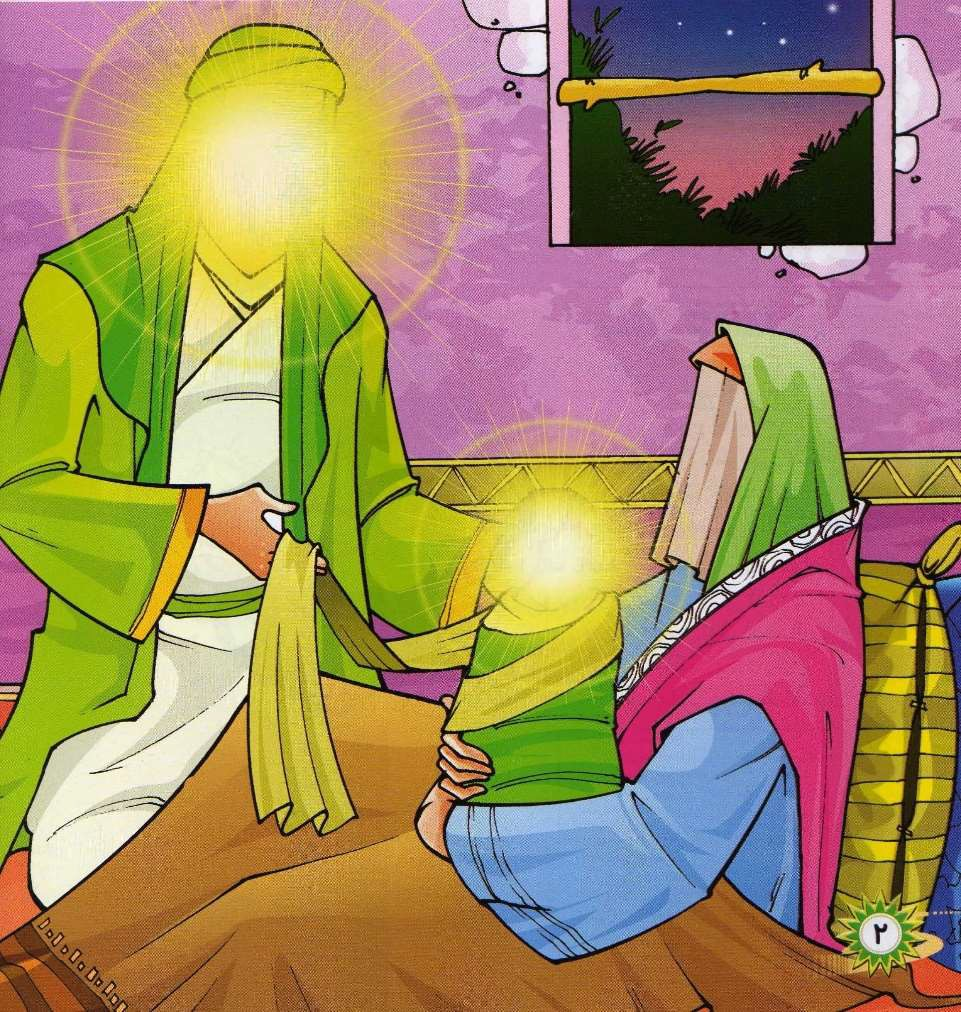
\includegraphics[width=6.3in,height=4.20208in]{media/image4.jpeg}

Selon la théologie musulmane, l'islam est la religion originelle de
l'humanité.VICTOR MOUSSA - STOCK.ADOBE.COM

\subsection{► Que dit la tradition ?}

Selon la théologie musulmane, l'islam est la religion originelle de
l'humanité.~\emph{« Tout homme est né musulman »,}~dit un hadith
attribué
au~\href{https://www.la-croix.com/sacralite-prophete-lislam-2020-11-06-1101123195}{\underline{prophète
Mohammed}}. L'homme est né pour adorer Dieu : certes, il a reçu une
dignité plus haute que les autres créatures, mais celle-ci est
conditionnée à sa soumission au Dieu unique. Plus un homme applique la
loi divine (\emph{charia}), plus il devient humain. Quant au « mécréant
» (\emph{kâfir}), qui refuse de suivre la charia, il se situe en quelque
sorte à un degré inférieur d'humanité.

Cette sévérité envers les non-musulmans s'appuie sur la lecture du texte
coranique qui s'est imposée à partir du IX\textsuperscript{e}~siècle,
lors de la transformation de l'islam en un empire soucieux de se
légitimer. Confortée par des hadiths rédigés à cette époque, elle
dépeint une vérité unique et non négociable. Elle insiste sur les
versets du Coran particulièrement virulents envers les polythéistes,
païens ou idolâtres, qualifiés d'\emph{« associateurs
»}~(\emph{mouchrikoun}) car ils « associent » à Dieu d'autres divinités.

Quant aux athées,~\emph{« ils appartiennent, selon la théologie
musulmane, à une catégorie de mécréance encore inférieure aux
polythéistes, aux juifs et aux chrétiens »,~}explique l'islamologue
Abdessamad Belhaj, chercheur au Centre interdisciplinaire d'études de
l'islam dans le monde contemporain de l'Université catholique de
Louvain. Même si des institutions comme le Haut Conseil des oulémas du
Maroc ou la Maison de la fatwa en Égypte considèrent que les apostats ne
peuvent plus être condamnés à mort, cette peine reste appliquée dans une
dizaine de pays, comme l'Afghanistan ou
la~\href{https://www.la-croix.com/Monde/Afrique/prisons-Mauritanie-calvaire-dun-apostat-2019-09-30-1201051050}{\underline{Mauritanie}}.

\subsection{ Pourquoi juifs et chrétiens bénéficient-ils d'un statut
spécifique ?}

Selon la tradition musulmane, chrétiens et juifs font l'objet d'un
traitement différent des autres non-musulmans : ils bénéficient dans le
droit islamique d'une protection juridique particulière (\emph{dhimma})
toutefois accompagnée d'injonctions humiliantes, comme l'interdiction de
monter à cheval ou de construire des lieux de culte dépassant ceux des
musulmans.
 

\emph{« Le Coran est très ambivalent au sujet des ``gens du Livre''
»,~}rappelle
l'historien~\href{https://www.la-croix.com/Culture/Livres-et-idees/historiens-decryptent-Coran-avant-lislam-2019-11-27-1201063090}{\underline{Guillaume
Dye}}, professeur à l'Université libre de Bruxelles (1). Selon la
sourate 5, juifs et chrétiens ne doivent pas être pris pour~\emph{«
alliés »~}(5, 51) mais, quelques versets plus loin, on lit qu'ils ne
seront~\emph{« point affligés »~}(5, 69). Les chrétiens se voient
reprocher de nier l'unicité de Dieu mais du respect est exprimé pour les
prêtres et les moines, qui~\emph{« ne s'enflent pas d'orgueil ».}

Selon une théologie dite de la falsification (\emph{tahrif}), les juifs
et les chrétiens ont altéré le message transmis par leurs prophètes
respectifs (Moïse, Jésus), message qui n'était autre que l'islam. Le
Coran, lui, corrige cette déviation en transmettant fidèlement le
message révélé à un ultime prophète, Mohammed. À Médine, celui-ci aurait
signé une~\emph{« Constitution »~}disposant que les juifs, notamment,
pouvaient pratiquer leur religion en sécurité, mais ces relations se
sont rapidement détériorées.

\subsection{► Quelles pistes pour une « théologie du pluralisme » ?}

Les attentats visant des « mécréants » en terrasse à Paris, les
persécutions contre les Yézidis ou les chrétiens en Irak, sont autant de
conséquences d'une lecture littéraliste du Coran encouragée par l'essor
du salafisme saoudien à partir des années 1970. D'autres lectures ont
pourtant existé dès les premiers siècles de l'islam. Contrairement à la
doctrine sunnite traditionnelle, l'exégèse rationaliste a par exemple
conclu très tôt à une~\emph{« égalité entre tous les êtres humains, tous
étant dotés de la même raison les rendant aptes à comprendre la parole
de Dieu »,~}rappelle l'islamologue Pierre Lory, directeur d'études à
l'École pratique des hautes études (EPHE).

Pour Abdessamad Belhaj, tout l'enjeu est aujourd'hui de refonder le
rapport à l'altérité sur la base de l'éthique, et de\emph{~« mettre
l'homme au cœur de la théologie »}. Pour cela, certaines valeurs
présentes dans l'islam gagneraient à être redécouvertes, comme celles du
soin, du don et du service à l'humanité, longtemps éclipsées selon lui
par l'autorité et la loyauté à la communauté musulmane ou à la tribu.

(1) Il a codirigé avec Mohammad Ali Amir-Moezzi, Le Coran des
historiens, 2019, Éd. du Cerf, 3~408~p., 89~€.

Faudra-t-il sauver les salafistes ?

Le gouvernement français a voulu lancer en octobre 2019 une offensive
contre l'islamisme et les courants radicaux, rapidement relayée par un
emballement médiatique qui a échappé à tout contrôle. Or, l'ennemi
désigné n'a nullement été identifié selon des termes juridiques, pas
plus que ses torts. On lui reproche sa piété rigoureuse, son voile, sa
pratique du jeûne de Ramadan, sa barbe fournie, son refus de toucher les
femmes, ce qui le rapproche dangereusement de n'importe quel fidèle
conservateur.

L'offensive vise donc une manière de concevoir la piété musulmane, et
nullement une qualification criminelle ou une atteinte à l'ordre public.
C'est dire que nous sommes confrontés à un « délit de sale gueule »,
lequel échappe à la tradition juridique républicaine, délit qui est
indiscernable, sans limite, extensible, mais politiquement pratique
auprès d'une opinion chauffée à blanc par les attentats et
l'immigration.

\subsection{Un engagement d'abord religieux}

Si l'islamiste ainsi décrit ressemble évidemment
au~\href{https://www.la-croix.com/Religion/Islam/Quest-salafisme-2018-10-14-1200975866}{\underline{salafiste}},
c'est oublier un peu vite que l'écrasante majorité des~\emph{salafi~}--
ceux qui sont attachés au modèle des « anciens » (les~\emph{salaf}),
c'est-à-dire les compagnons du Prophète -- se veulent quiétistes : leur
mode d'action est la prédication et l'action missionnaire
(la~\emph{da`wa}). Le salafiste souhaite d'abord vivre un islam épuré et
intégriste -- au sens d'intégral -- dans le cadre de sa famille et de sa
communauté.

Ce mouvement est distinct d'un engagement politique, de sorte que les
salafistes sont rarement liés aux Frères musulmans, qui eux forment un
mouvement politique. Si la matrice religieuse et idéologique du
salafisme imprègne les mentalités djihadistes, elle ne se confond pas
avec celles-ci, ni dans la pensée, ni dans les faits. La radicalisation
concerne donc à des degrés différents et sous des formes incomparables
les sympathisants du salafisme et les partisans du djihadisme de Daech.
Les premiers ont un engagement d'abord religieux, tandis que les autres
sont mus à la fois par la volonté de puissance, des facteurs politiques,
sociaux et religieux.

\subsection{L'autodidacte de l'islam présente plus de risques que le
salafiste}

L'hostilité des salafistes envers les courants djihadistes a été prouvée
à de nombreuses reprises par des déclarations publiques et surtout en
fournissant du renseignement de qualité auprès des services de police.
Le meilleur ennemi du terroriste est souvent le~\emph{salafi}, et
l'autodidacte de l'islam présente plus de risques que le salafiste.

En outre, le salafisme n'a pas été désavoué par les représentants du
culte musulman pour la simple raison que ce courant n'est pas une
idéologie : il faudrait donc lui enlever son~\emph{isme}~final et
l'appeler, selon la tradition religieuse, la~\emph{salafiya~}; il s'agit
d'un vieux courant légitime de l'islam, qui a fourni des générations
d'imams et de lettrés attachés au sens littéral du Coran et de la Sunna.

\subsection{Un « écosystème » étroit mais rassurant}

Il est évident que le salafisme représente une alternative culturelle et
sociale au modèle français, modèle égalitaire, inclusif, ouvert (au
moins en théorie). Les quelques salafi que j'ai connus -- des convertis
à 25 ou 30 \% d'entre eux -- vivaient dans un étroit triangle
géographique. Parce qu'ils souhaitent faire les cinq prières à leur
heure, sans les décaler, et ce dans une salle de prière, ils sont
contraints de vivre et de travailler non loin d'une mosquée. Ils passent
ainsi de leur habitation au lieu de travail et à la salle de prière,
lesquels se situent nécessairement dans un « écosystème » étroit mais
rassurant. Ils ne peuvent guère être exigeants sur le plan
professionnel.

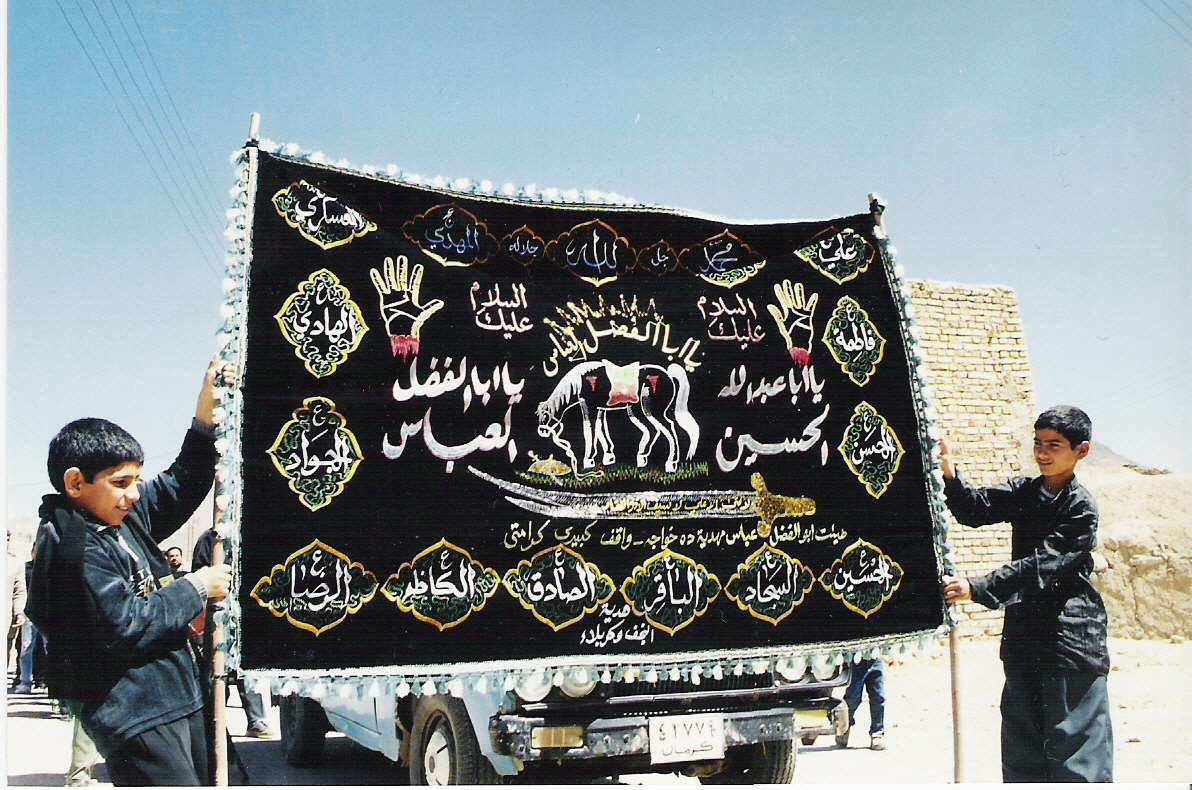
\includegraphics[width=1.97917in,height=1.40972in]{media/image6.jpeg}

\href{https://www.la-croix.com/Religion/Le-Coran-peut-etre-interprete-2021-01-25-1201136852}{Le
Coran peut-il être interprété ?}

Le salafisme, qui représente au moins 40 000 individus, est socialement
dangereux car il impose l'auto-ségrégation, le refus des contacts avec «
ceux qui n'en sont pas ». C'est la raison pour laquelle les spécialistes
des questions de sécurité se refusent à les impliquer dans la lutte
contre le djihadisme. Salafistes et terroristes participeraient à une
même matrice intellectuelle, celle du bien contre le mal, une sorte de
vision sectaire du monde. La différence vient du rapport à la violence :
assumé chez les djihadistes, rejeté chez les salafistes. Leur
fondamentalisme présente l'avantage d'une certaine forme de morale : à
Sartrouville les quartiers salafisés ont vu s'effondrer la toxicomanie
et la délinquance, avec le soutien de la mairie.

\subsection{Confondre l'approche culturelle avec la lutte contre le
terrorisme}

Ces courants ne peuvent être incriminés sur le plan sécuritaire. On
confond donc l'approche culturelle avec la lutte contre le terrorisme. À
moins de changer tout le droit européen, la première doit être menée par
l'éducation, la philosophie, la raison, le débat ; quant à la seconde
elle doit s'appuyer sur le droit et sur des qualifications pénales, et
non sur de vagues impressions de « radicalisation », notion qui n'a
toujours pas été appréhendée de façon rigoureuse en termes sociologiques
et psychologiques.

Comme la guerre d'Algérie nous l'enseigne, une telle manière de
concevoir l'action politique va aboutir à l'effet inverse de celui
recherché : le renforcement de la méfiance collective, le repli
communautaire du côté musulman, l'action violente du côté des « anti »,
et, finalement, la fragmentation sociale et l'insécurité.

\subsection{Islam : les fumées de la radicalisation}

Olivier Hanne, médiéviste (université de Poitiers), chercheur en
islamologie, estime qu'il est très difficile de définir le parcours type
d'une personne radicalisée. Le dernier de trois articles consacrés à
l'islam en France. 
 

Qui parle d'islam aujourd'hui pense aussitôt à la radicalisation. En
2015, on estimait entre 8 000 et 10 000 le nombre de Français
radicalisés. Leurs profils sont si variés qu'il est difficile de donner
des catégories fixes : les mineurs représentent 25 \% des cas, les
femmes 27 \%, les personnes signalées sont plutôt jeunes (entre 16 et 30
ans), leur niveau scolaire est généralement faible, même si l'on
rencontre des diplômés.

La plupart travaillent. Internet représente pour tous ces individus un
passage obligé, même s'il se concrétise différemment : terrain initial
de la radicalisation, facteur de renforcement ou vecteur unique de
l'expression radicale, le partage des contenus djihadistes sur Internet
n'a pas du tout la même fonction chez une adolescente connectée, un
salafiste convaincu et un combattant expérimenté déjà parti en Syrie.

\subsection{Les autorités font feu de tout bois}

De toute évidence, l'attraction pour la radicalité religieuse n'est pas
nécessairement liée à un phénomène de rupture sociale. Les failles de la
société contemporaine (éclatement des familles, déclin des autorités et
des idéologies, chômage, ghettoïsation) créent un terreau facilitateur,
mais nullement déterminant. La frustration individuelle alimente le
recours à des convictions extrêmes, voire le passage à l'acte
terroriste, mais n'est qu'un facteur parmi tant d'autres.

Les autorités font feu de tout bois pour tenter de faire face à une
radicalisation multiforme. En avril 2015, le premier ministre français,
Manuel Valls, annonçait l'ouverture d'une dizaine de centres de
prévention de la radicalisation, dont la plupart furent un échec. Des
sites Internet officiels sont créés et proposent des fiches techniques
contre la radicalisation et le terrorisme, dont le contenu est souvent
simple, voire binaire. Ainsi sur le site
français~\emph{stop-djihadisme.gouv.fr}, un bandeau intitulé «
Radicalisation djihadiste, les premiers signes qui peuvent alerter »
énonce pêle-mêle : « ils se méfient des anciens amis qu'ils considèrent
maintenant comme des impurs » ; « ils changent brutalement leurs
habitudes alimentaires » ; « ils arrêtent d'écouter de la musique car
elle les détourne de leur mission » ; « ils ne regardent plus la
télévision et ne vont plus au cinéma ». Autant de signes extérieurs qui
se rapprochent de l'adolescente anorexique\ldots{} L'efficacité de ces
dispositifs a d'ailleurs été très contestée dès 2015.

\subsection{L'État, tenté d'être omniprésent}

Toute l'entreprise de déradicalisation définit en creux le modèle
positif occidental : monde de loisirs, de consommation, d'épanouissement
personnel et professionnel. Le vocabulaire de la radicalisation masque
le rejet de ce modèle culturel. Et les pouvoirs publics d'hésiter à
appeler leur objectif par son vrai nom : le reconditionnement mental.

Le danger de la déradicalisation se situe dans l'élargissement des
intrusions de l'État : en voulant réinsérer, l'État pénètre dans
l'intimité des individus afin de redéfinir le religieux et lui redonner
une place acceptable. Or, l'État a-t-il compétence pour définir ce
qu'est l'islam, le « bon » islam ? Ne sachant cerner la menace, l'État
est tenté d'être omniprésent, sans en avoir la capacité légale. La
déradicalisation pourrait relever de la posture intellectuelle.

Le problème vient sans doute des hésitations du vocabulaire. Car,
après-tout, qu'est-ce que la radicalisation ? Au
XIX\textsuperscript{e}~le mot anglais~\emph{radical}~était employé pour
désigner les partis politiques britanniques exigeant une réforme
démocratique libérale. Transféré tel quel en France, on l'appliqua aux
partis de gauche, laïques et libéraux qui voulaient réformer la société.

\subsection{Réactions épidermiques}

Le verbe « radicaliser » fut employé régulièrement dans les années
1960-1970 dans une acception politique avec l'idée de « devenir plus
intransigeant, se durcir » ou « plus extrême ». Le premier sens était
donc politique et pas nécessairement négatif. Se déradicaliser était un
synonyme pour « se compromettre ». Appliqué à l'islamisme, le verbe
impose une redéfinition complète des termes : à partir de quand
juge-t-on l'islam intransigeant ou extrême ? par rapport à quelle norme
? à quelle moyenne ?

Les réactions épidermiques qui ont suivi le meurtre de l'enseignant de
Conflans-Sainte-Honorine en octobre 2020 sont tristement révélatrices :
les imams doivent s'exprimer ! les musulmans doivent désavouer le
terrorisme et faire allégeance à la France ! Mais quand ils le font,
c'est encore insuffisant, déloyal et mensonger. Le gouvernement proposa
même qu'ils prient pour la République au cours de la prière collective
du vendredi. Nos références sur la question religieuse restent
tragiquement celles de la Révolution française : comme il y eut les «
prêtres jureurs », adhérant à la loi, contre les « prêtres réfractaires
», obstinés dans leur obéissance à Rome, de la même façon il nous faut
des « imams jureurs », intimement républicains. L'État se retrouve donc
juge des reins et des cœurs.

%\bibliography{Theo}
%\bibliographystyle{siam}
\printbibliography

\listoftheorems[ignoreall,show={Def}]
Les courants contemporains de l’islam Glossaire général

\mn{Vérifier les termes}

bid‘a : innovation ; pratique « déviante ».

da‘wa : invitation ; prédication – appel à la conversion (dans les deux sens).

fasiq : pécheur ; mauvais musulman.

fiqh : compréhension ; corpus du droit musulman.

fitna: discorde, querelle ; conflit interne au monde musulman.

hadith : récit d’un dire ou faire du Prophète, rapporté par ses compagnons.

hajj : pèlerinage annuel à La Mecque.

hijra (héjire) : « exode » - départ de Mahomet pour Médine (622).

‘ibadat : culte ; partie du droit traitant du culte.

ijma‘ : consensus ; consensus des ulama sur un point de droit.

ijtihad : effort ; effort d’interprétation du Coran.

imam : chef suprême de la communauté musulmane ; successeur du Prophète, utilisé communément par les chiites pour Ali et ses descendants.

islah : réforme.

isnad : chaîne ; chaîne de transmission des hadiths.

jihad : lutte ; soit intérieure, contre ses propres faiblesses ; soit extérieure, contre les ennemis de la communauté musulmane.

ka‘aba : monument cubique noir situé au centre de la grande mosquée de La Mecque ; selon les musulmans, désigne l’emplacement du premier autel élevé par Abraham pour le Dieu unique. Point vers lequel se dirigent les musulmans pour prier.

kafir : infidèle, mécréant

khalifa (calife) : successeur, représentant ; successeur du Prophète et chef de la communauté musulmane (sunnisme).

madrasa : école ; lieu où est assuré la transmission du savoir religieux.

mihrab : niche indiquant la direction de La Mecque dans une mosquée.
 
mu‘amalat : relations ; partie du droit traitant des relations humaines.

qibla : orientation de la prière rituelle (salat), correspondant à la direction de La Mecque.

qiyas : raisonnement par analogie (domaine du droit)

salat : prière rituelle.

seyyed : prince, chef ; descendant du Prophète par Hossein ou Hassan, fils d’Ali.

shari‘a : sentier, voie ; loi divine.

sheykh (cheykh) : vieil homme ; chef d’une tribu ; chef religieux ; personne à la tête d’une congrégation soufie, ayant la capacité de guider ses disciples.

shirk : associationnisme : fait d’adorer d’autres êtres en dehors de Dieu.

shura : principe de consultation soufi : mystique musulman sourate : chapitre du Coran
sunna : coutume ; pratiques du Prophète et de la première communauté musulmane, faisant autorité pour guider le mode de vie des croyants et déterminer la loi religieuse.

tafsir : commentaire du Coran.

tajdid : renouveau (=>mujaddidi : qui renouvelle)

taqlid : imitation ; imitation stérile des anciens (par opposition à l’ijtihad).

tariqa : voie : confrérie soufie.

tawhid : unicité (divine). Dogme fondamental de l’islam.

ulama (oulémas) : terme collectif pour désigner les lettrés musulmans.

umma : peuple ou communauté ; communauté islamique dans son ensemble.

waqf : bien immobilier ou foncier dit « de-main-morte », dépendant des institutions religieuses.

zakat : aumône rituelle, obligatoire pour les croyants.

%\listoftheorems


\end{document}